\documentclass[dvipsnames]{beamer}
%Text
\usepackage[utf8]{inputenc}
\usepackage[english]{babel}
\usepackage{anyfontsize}
\usepackage{xcolor}
\newcommand{\myurl}[2][blue]{{\color{#1}\url{#2}}}
%Theme
\usetheme[pageofpages=of,% String between current/total page counts
          bullet=circle,% Use circles instead of squares for bullets.
          titleline=true,% Show a line below the frame title.
          alternativetitlepage=true,% Use the fancy title page.
          titlepagelogo=../nontext/images/mcmaster_logo,% Logo for title
          %watermark=../nontext/images/mcmaster_logo,% logo in every page.
          watermarkheight=1px,% Height of the watermark.
          watermarkheightmult=1,%watermakr x bigger than watermarkheight
          ]{Torino}
%Graphics
\usepackage{graphicx}
\graphicspath{{../nontext/figures/}{../nontext/images/}}
\usepackage[section]{placeins} %for FloatBarrier
\def\Put(#1,#2)#3{\leavevmode\makebox(0,0){\put(#1,#2){#3}}}
\usepackage{multicol}
%Refernces
\usepackage[natbib=true,
            bibencoding=utf8,
            style=authoryear,
            backend=biber,
            %autocite=superscript,
            sorting=none,
            useprefix=true]{biblatex}
\addbibresource{../refs.bib}
\usepackage[absolute,overlay]{textpos}
%Tikz
\usepackage{tikz}% for flow chart
\usepackage{moresize} %for ssmall font size
\usepackage{tikz-network}
\usetikzlibrary{calc,shapes,arrows,positioning,fit,quotes,shapes.misc}% for flow chart
%Styles
\tikzstyle{block} = [circle,
                     fill=green!20,
                     text centered,
                     font=\ssmall,
                     text width=1.5cm,
                     rounded corners,
                     draw]
\tikzstyle{slock} = [circle,
                     fill=red!20,
                     font=\ssmall,
                     text width=1.5cm,
                     text centered,
                     rounded corners,
                     draw]
\tikzstyle{flock} = [circle,
                     fill=blue!20,
                     font=\ssmall,
                     text width=1.5cm,
                     text centered,
                     rounded corners,
                     draw]
\tikzstyle{line} = [draw, -latex']
\newcommand{\Checkmark}{$\mathbin{\tikz [x=2.4ex, y=2.4ex, line width=.2ex, green] \draw (0,1) -- (1,0) -- (3,3);}$}
%Progress bar
%setup
\definecolor{pbgreen}{RGB}{98,189,25}% color for the progress bar and the circle
\renewcommand{\inserttotalframenumber}{\pageref{lastslide}}
\makeatletter
\def\progressbar@progressbar{} % the progress bar
\newcount\progressbar@tmpcounta% auxiliary counter
\newcount\progressbar@tmpcountb% auxiliary counter
\newdimen\progressbar@pbht %progressbar height
\newdimen\progressbar@pbwd %progressbar width
\newdimen\progressbar@rcircle % radius for the circle
\newdimen\progressbar@tmpdim % auxiliary dimension

\progressbar@pbwd=\linewidth
\progressbar@pbht=1pt
\progressbar@rcircle=2.5pt

%the progress bar
\def\progressbar@progressbar{%

    \progressbar@tmpcounta=\insertframenumber
    \progressbar@tmpcountb=\inserttotalframenumber
    \progressbar@tmpdim=\progressbar@pbwd
    \multiply\progressbar@tmpdim by \progressbar@tmpcounta
    \divide\progressbar@tmpdim by \progressbar@tmpcountb

  \begin{tikzpicture}
    \draw[pbgreen!30,line width=\progressbar@pbht]
      (0pt, 0pt) -- ++ (\progressbar@pbwd,0pt);

    \filldraw[pbgreen!30] %
      (\the\dimexpr\progressbar@tmpdim-\progressbar@rcircle\relax, .5\progressbar@pbht) circle (\progressbar@rcircle);

    \node[draw=pbgreen!30,text width=3.5em,align=center,inner sep=1pt,
      text=pbgreen!70,anchor=east] at (0,0) {\insertframenumber/\inserttotalframenumber};
  \end{tikzpicture}%
}
%add bar
\addtobeamertemplate{headline}{}
{%
  \begin{beamercolorbox}[wd=\paperwidth,ht=4ex,center,dp=1ex]{white}%
    \progressbar@progressbar%
  \end{beamercolorbox}%
  \vspace{-0.25in}
}
\makeatother
%Dont Count backup Slide Numbers
\newcommand{\backupbegin}{
       \newcounter{framenumbervorappendix}
          \setcounter{framenumbervorappendix}{\value{framenumber}}
}
\newcommand{\backupend}{
     \addtocounter{framenumbervorappendix}{-\value{framenumber}}
        \addtocounter{framenumber}{\value{framenumbervorappendix}}
}
%Abbreviations
\usepackage{acro}
%otu
\DeclareAcronym{otu}{
    short = OTU,
    long  = Operation Taxonomic Unit
}
%pa
\DeclareAcronym{pa}{
    short = P/A,
    long  = Presence/Absence,
}
%mge
\DeclareAcronym{mge}{
    short = MGE,
    long  = Mobile Genetic Element
}
%ecoli
\DeclareAcronym{ecoli}{
    short = \textit{E. coli},
    long  = \textit{Escherichia coli}
}
%cas
\DeclareAcronym{cas}{
    short = Cas,
    long  = CRISPR-associated protein
}
%crsp
\DeclareAcronym{crsp}{
    short = CRISPR,
    long  = Clustered Regularly Interspaced Short Palindromic Repeat
}
%crspc
\DeclareAcronym{crspc}{
    short = CRISPR-Cas,
    long  = CRISPR-Cas
}
%HGT
\DeclareAcronym{hgt}{
    short = HGT,
    long = Horizontal Gene Transfer
}
%Title
\title{{\fontsize{40}{50}\selectfont Is Sharing Caring?}}
\subtitle{\vspace{-0.2in}Elucidating the Effects of the Presence of CRISPR-Cas Systems on Rates of Horizontal Gene Transfer Using Network Analysis\vspace{0.1in}}
\date{April 10, 2019}
\author{Siddharth Reed\\
        Biology Undergraduate Symposium
       }
\institute{Golding Lab,\\
           Biology Department,\\
           McMaster University
          }

\begin{document}
\watermarkoff %theme has watermark on every slide, turning that off
%Title Slide
\begin{frame}[t,plain]
    \titlepage
\end{frame}
%Table Of Contents
\begin{frame}[plain]{Table of Contents}
  \setbeamertemplate{section in toc}[sections numbered]
  \tableofcontents[hideallsubsections]
  \addtocounter{framenumber}{-1}
\end{frame}
\section{Background}
\begin{frame}[fragile,plain]{}%Phylonets}
    \begin{center}
        \Huge \textcolor{OliveGreen}{Networks}
    \end{center}
    \addtocounter{framenumber}{-1}
\end{frame}
\begin{frame}[fragile]{What is A Network?}
\begin{columns}
    \begin{column}{0.5\textwidth}
        \begin{figure}[htb!]\onslide<2->
            \makebox[\textwidth][c]{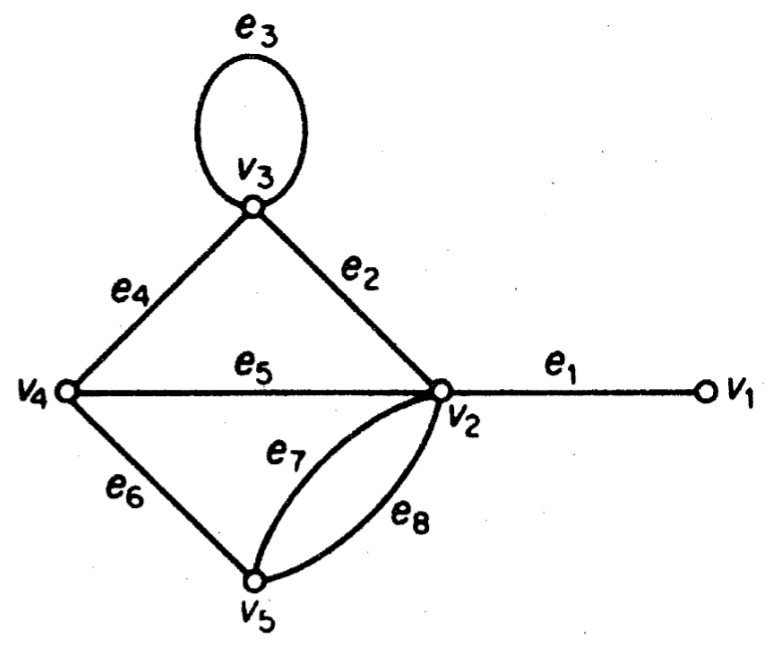
\includegraphics[width=0.8\linewidth]{graphExample_bondy.png}}
        \end{figure}
        \autocite{bondy}
    \end{column}
    \begin{column}{0.5\textwidth}
        \begin{itemize}
            \item<2-> Useful mathematical abstraction of real world system
            \item<3-> Nodes represent objects
            \item<4-> Edges represent relationshisps
            \item<5-> Nodes and edges can have attributes
            \item<6-> \textbf{Nodes are \ac{otu}s, edges are inferred HGT rates}
        \end{itemize}
    \end{column}
\end{columns}
\end{frame}
\begin{frame}[fragile,plain]{}%HGT}
    \begin{center}
        \Huge \textcolor{OliveGreen}{Horizontal Gene Transfer}
    \end{center}
    \addtocounter{framenumber}{-1}
\end{frame}
\begin{frame}[fragile]{Horizontal Gene Transfer Mechanisms}
    \begin{columns}
    \begin{column}{0.5\textwidth}
        \begin{figure}[htb!]\onslide<1->
            \makebox[\textwidth][c]{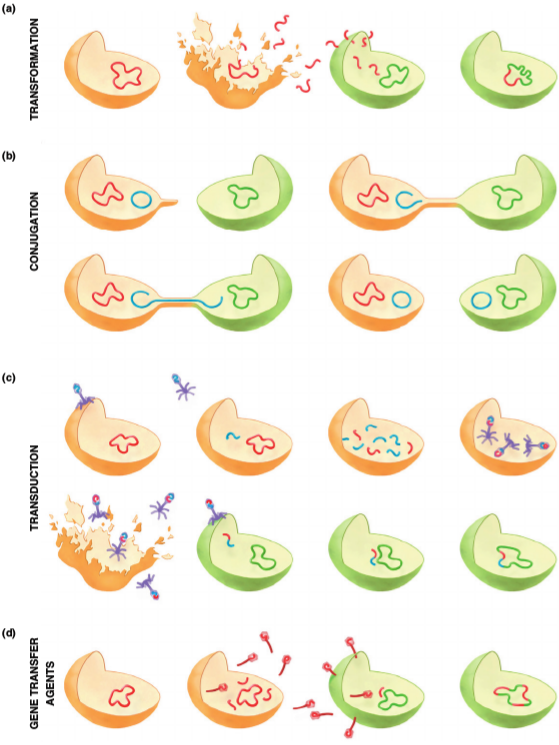
\includegraphics[width=0.8\linewidth]{hgt_mechanisims_trendslgt.png}}
            \autocite{trendslgt}
        \end{figure}
    \end{column}
    \begin{column}{0.5\textwidth}
        \begin{itemize}
            \item<2-> Transformation: Incorporation of free-floating DNA into the genome \autocite{trendslgt}
            \item<3-> Conjugation: Transfer of DNA through cell-cell connections \autocite{trendslgt}
            \item<4-> Transduction: Transfer of DNA through phage \autocite{trendslgt}
            %\item<5-> \textbf{CRISPR-Cas directly affects \ac{hgt}} \autocite{trendslgt}
        \end{itemize}
    \end{column}
    \end{columns}
\end{frame}
\begin{frame}[fragile,plain]{}%CRISPR-Cas Systems}
    \begin{center}
        \Huge \textcolor{OliveGreen}{CRISPR-Cas systems}
    \end{center}
    \addtocounter{framenumber}{-1}
\end{frame}
\begin{frame}[fragile]{What Are They?}
    \begin{columns}
    \begin{column}{0.5\textwidth}
        \begin{itemize}
            \item<2-> Adaptive Bacterial Immune System
            \item<3-> Failed “infection” $\to$ spacer acquisition $\to$ targeted degredation for next “infection”
            \item<4-> Protects against foreign DNA
            \item<5-> Requires Cas proteins and CRISPR loci
            \item<6-> $45\%$ of bacteria have CRISPR loci $(n=6782)$ \autocite{crispdb}
        \end{itemize}
    \end{column}
    \begin{column}{0.5\textwidth}
        \begin{figure}[htb!]\onslide<2->
            \makebox[\textwidth][c]{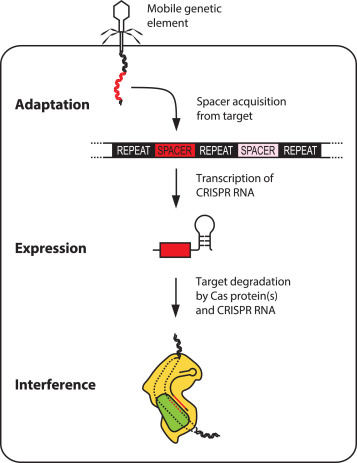
\includegraphics[width=0.8\linewidth]{CRISPR-immunity_crispgen.jpg}}
            \autocite{crispgen}
        \end{figure}
    \end{column}
    \end{columns}
\end{frame}
\begin{frame}[fragile,plain]{}%Do  They?}
    \begin{center}
        \Huge \textcolor{OliveGreen}{Do CRISPR Systems Affect Horizontal Gene Transfer?}
    \end{center}
    \addtocounter{framenumber}{-1}
\end{frame}
\begin{frame}[fragile]{}%Yes}
    \begin{center}
        \Huge Yes
    \end{center}
\end{frame}
\begin{frame}[fragile]{Previous Findings}
    \begin{itemize}
        \item<2-> Gophna et al. (2015) found no relation between the presence of \ac{crsp} systems and HGT over short evolutionary timescales
        \begin{itemize}
            \item<3-> Assume all singletons arose from HGT
            \item<4-> Used GC\% to identify HGT
        \end{itemize}
        \item<5-> Contradicted by a former undergraduate thesis student
        \begin{itemize}
            \item<6-> Can see inhibitory effects of CRIPSR on HGT over short evolutionary time scales
            \item<7-> Higher gene indel rates for CRISPR containing \ac{otu}s than non-CRISPR containing outgroups
        \end{itemize}
    \end{itemize}
\end{frame}
\section{My Project}
\begin{frame}[fragile,plain]{}%My Project}
    \begin{center}
        \Huge \textcolor{OliveGreen}{My Project}
    \end{center}
    \addtocounter{framenumber}{-1}
\end{frame}
\begin{frame}[fragile]{Objectives}
    \onslide<2-> \begin{block}{Within Network Comparisons}
        For genera with CRISPR containing \ac{otu}s, compare the node statistics of CRIPSR containing \ac{otu}s to non-CRISPR containing \ac{otu}s.
    \end{block}
%    \onslide<3-> \begin{block}{Between Network Comparisons}
%        For genera with no CRISPR containing strains, compare the network statistics of mixed to non-CRISPR-containing networks.
%    \end{block}
    \onslide<3-> \begin{block}{Gene Indel Rates vs. Network Statistics}
        Compare gene Indel rates to node/network statistics for CRISPR containing and non-CRISPR containing \ac{otu}s
    \end{block}
\end{frame}
\begin{frame}[fragile]{Workflow (Per Genus)}
\begin{center}
    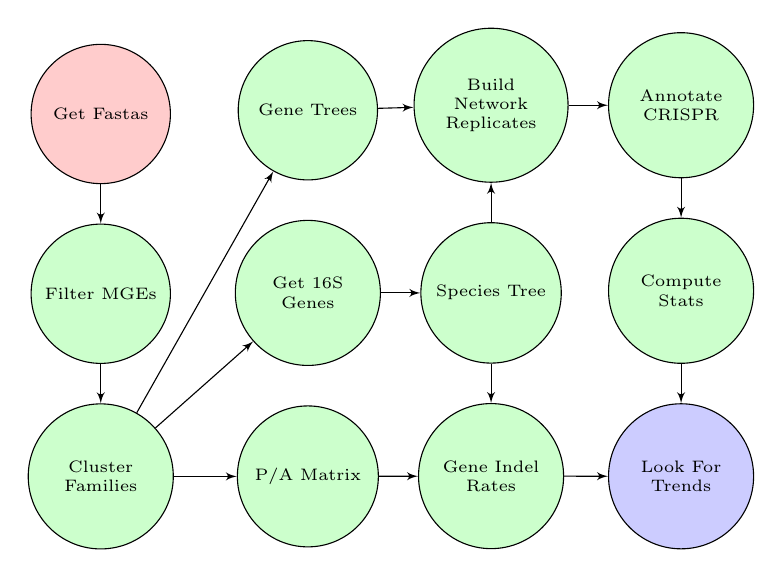
\begin{tikzpicture}
        % boxes
        \onslide<1->  \node [slock]                       (node1)  {Get Fastas};
        \onslide<2->  \node [block,below=0.5cm of node1]  (node2)  {Filter MGEs};
        \onslide<3->  \node [block,below=0.5cm of node2]  (node3)  {Cluster Families};
        \onslide<6->  \node [block,right=0.8cm of node3]  (node4)  {P/A Matrix};
        \onslide<4->  \node [block,above=0.5cm of node4]  (node5)  {Get 16S Genes};
        \onslide<8->  \node [block,above=0.5cm of node5]  (node6)  {Gene Trees};
        \onslide<5->  \node [block,right=0.5cm of node5]  (node7)  {Species Tree};
        \onslide<7->  \node [block,below=0.5cm of node7]  (node8)  {Gene Indel Rates};
        \onslide<9->  \node [block,above=0.5cm of node7]  (node9)  {Build Network Replicates};
        \onslide<10-> \node [block,right=0.5cm of node9]  (node10)  {Annotate CRISPR};
        \onslide<11-> \node [block,below=0.5cm of node10] (node11) {Compute Stats};
        \onslide<12-> \node [flock,below=0.5cm of node11] (node12) {Look For Trends};
        %lines
        \onslide<2->  \path [line] (node1) -- (node2);
        \onslide<3->  \path [line] (node2) -- (node3);
        \onslide<4->  \path [line] (node3) -- (node5);
        \onslide<5->  \path [line] (node5) -- (node7);
        \onslide<6->  \path [line] (node3) -- (node4);
        \onslide<7->  \path [line] (node4) -- (node8);
        \onslide<7->  \path [line] (node7) -- (node8);
        \onslide<8->  \path [line] (node3) -- (node6);
        \onslide<9->  \path [line] (node6) -- (node9);
        \onslide<9->  \path [line] (node7) -- (node9);
        \onslide<10-> \path [line] (node9) -- (node10);
        \onslide<11-> \path [line] (node10) -- (node11);
        \onslide<12-> \path [line] (node11) -- (node12);
        \onslide<12-> \path [line] (node8) -- (node12);
    \end{tikzpicture}
\end{center}
\end{frame}
\section{Results}
\begin{frame}[fragile,plain]{}
    \begin{center}
        \Huge \textcolor{OliveGreen}{Results}
    \end{center}
    \addtocounter{framenumber}{-1}
\end{frame}
\begin{frame}[fragile]{Example “Consensus” Network}
    \vspace{-0.05in}
    \makebox[\textwidth][c]{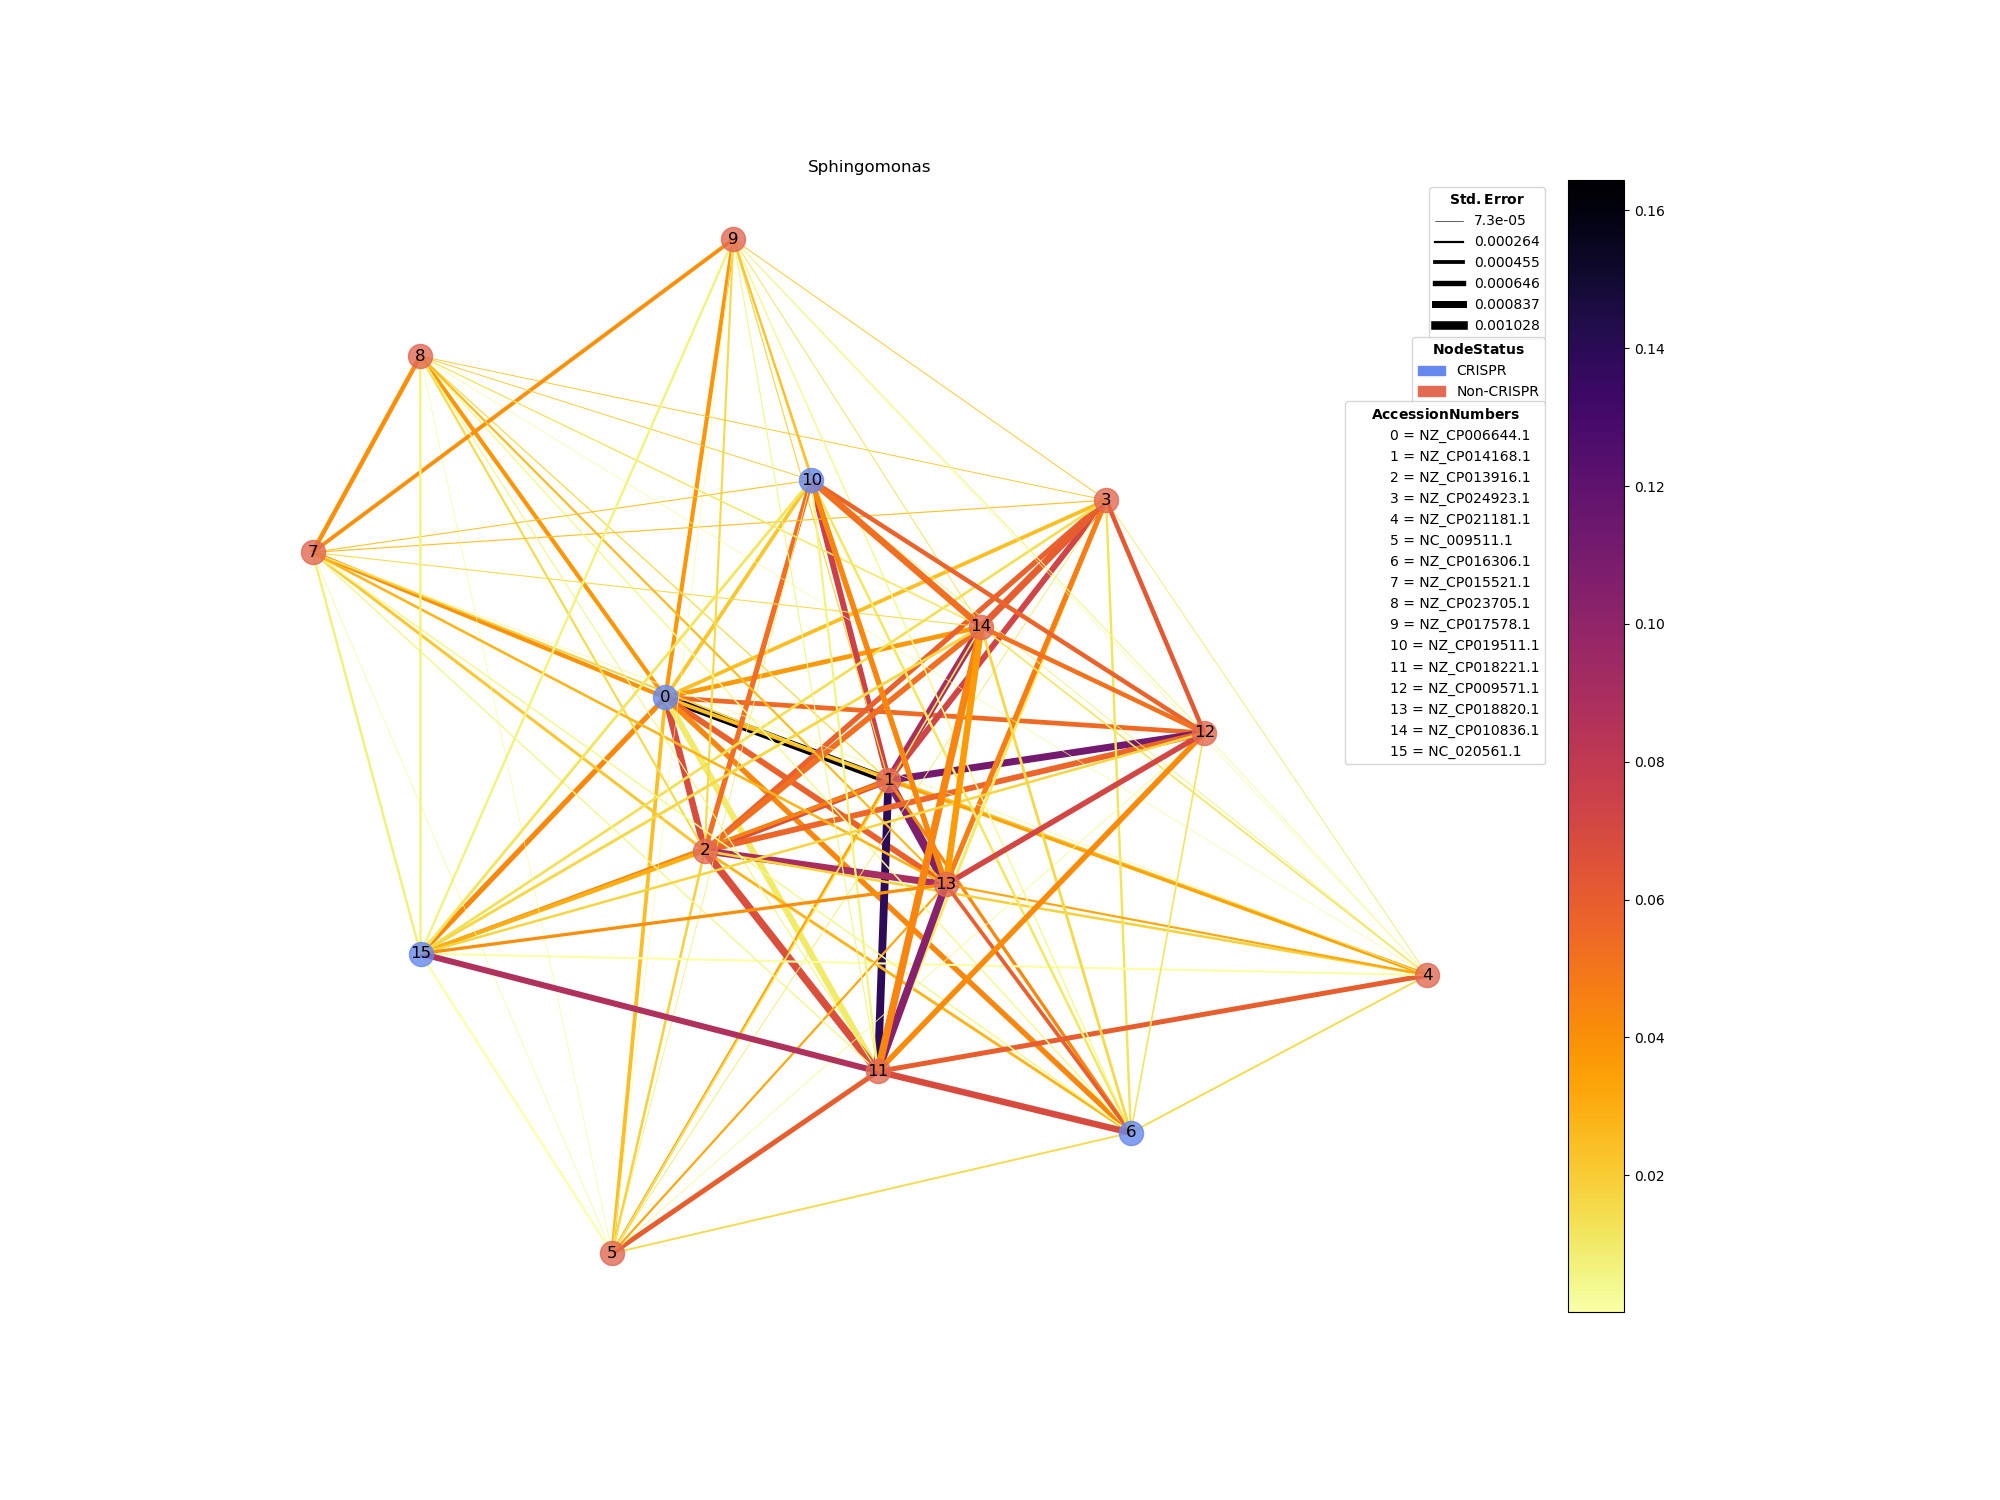
\includegraphics[width=\linewidth]{network.png}}
\end{frame}
\begin{frame}[fragile]{Mean Node Degree}
    \begin{figure}[htb!]
        \makebox[\textwidth][c]{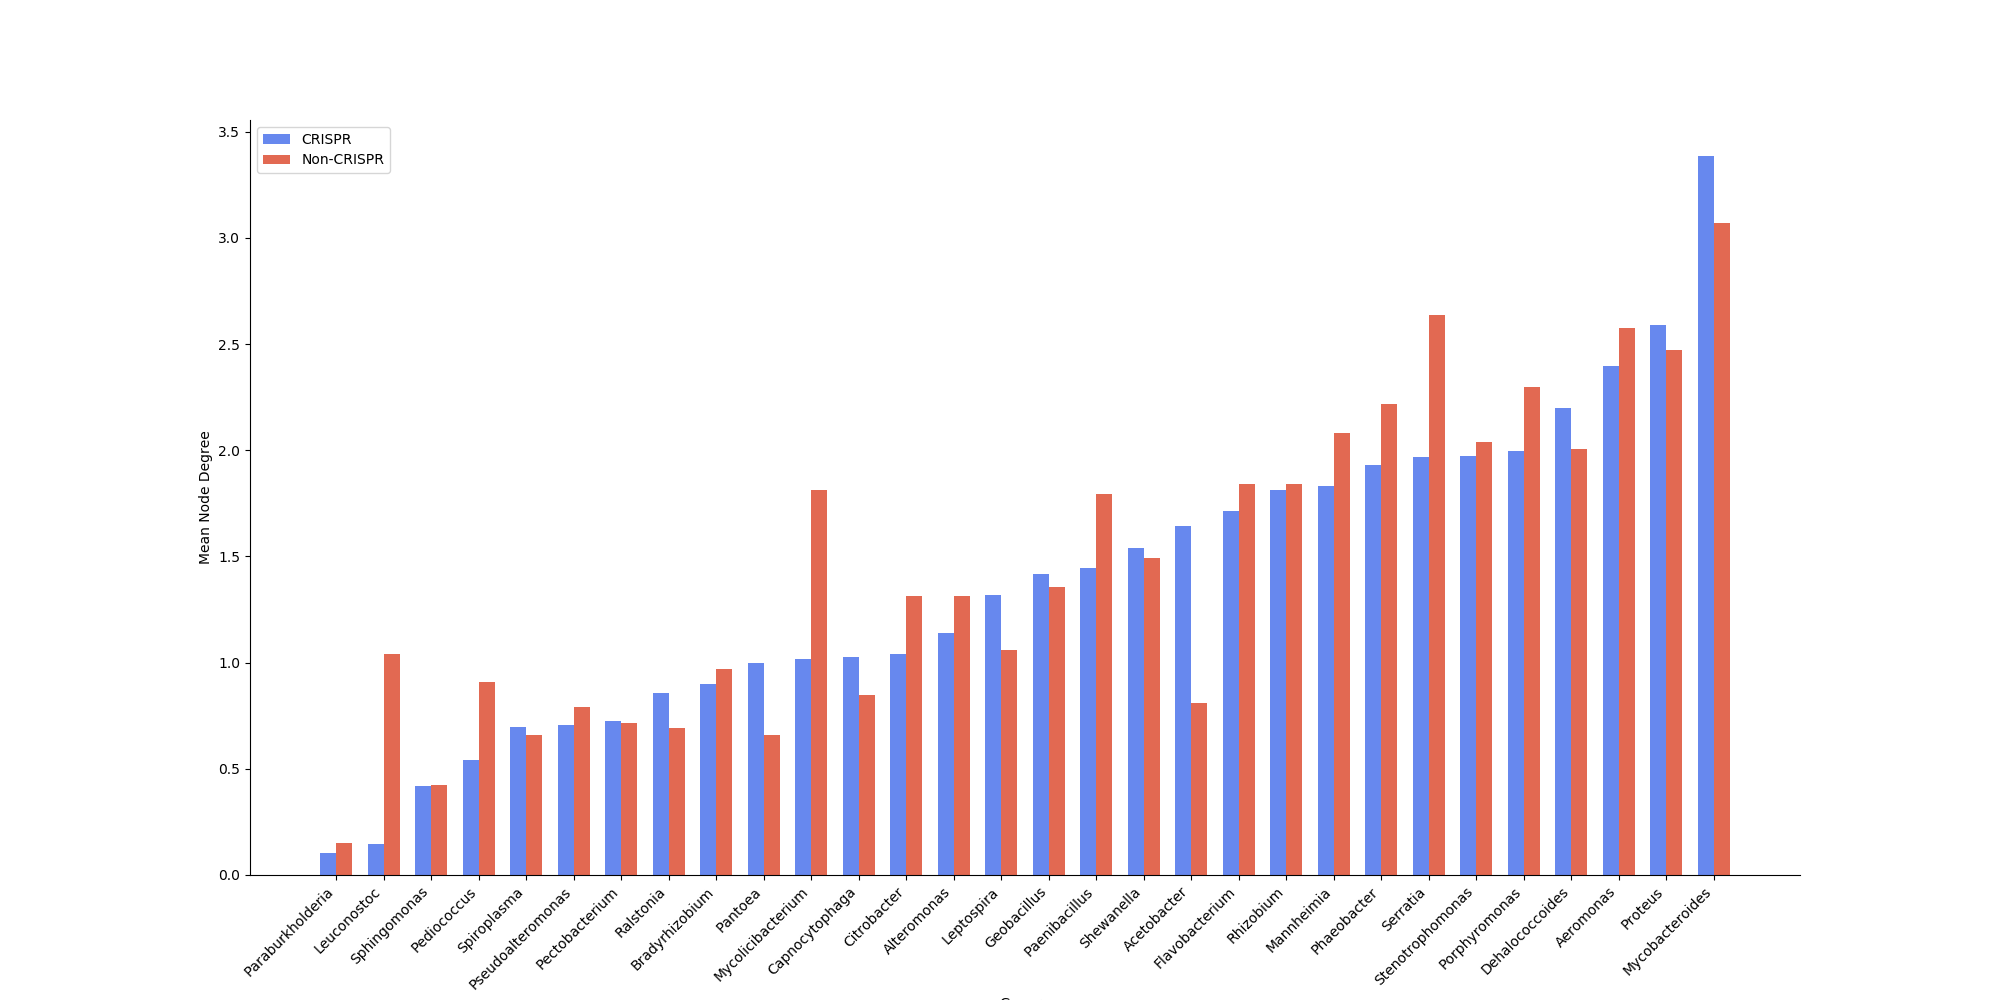
\includegraphics[width=1.2\linewidth]{c_nc_deg_bar.png}}
    \end{figure}
\end{frame}
\begin{frame}[fragile]{Gene Indel Rates}
    \makebox[\textwidth][c]{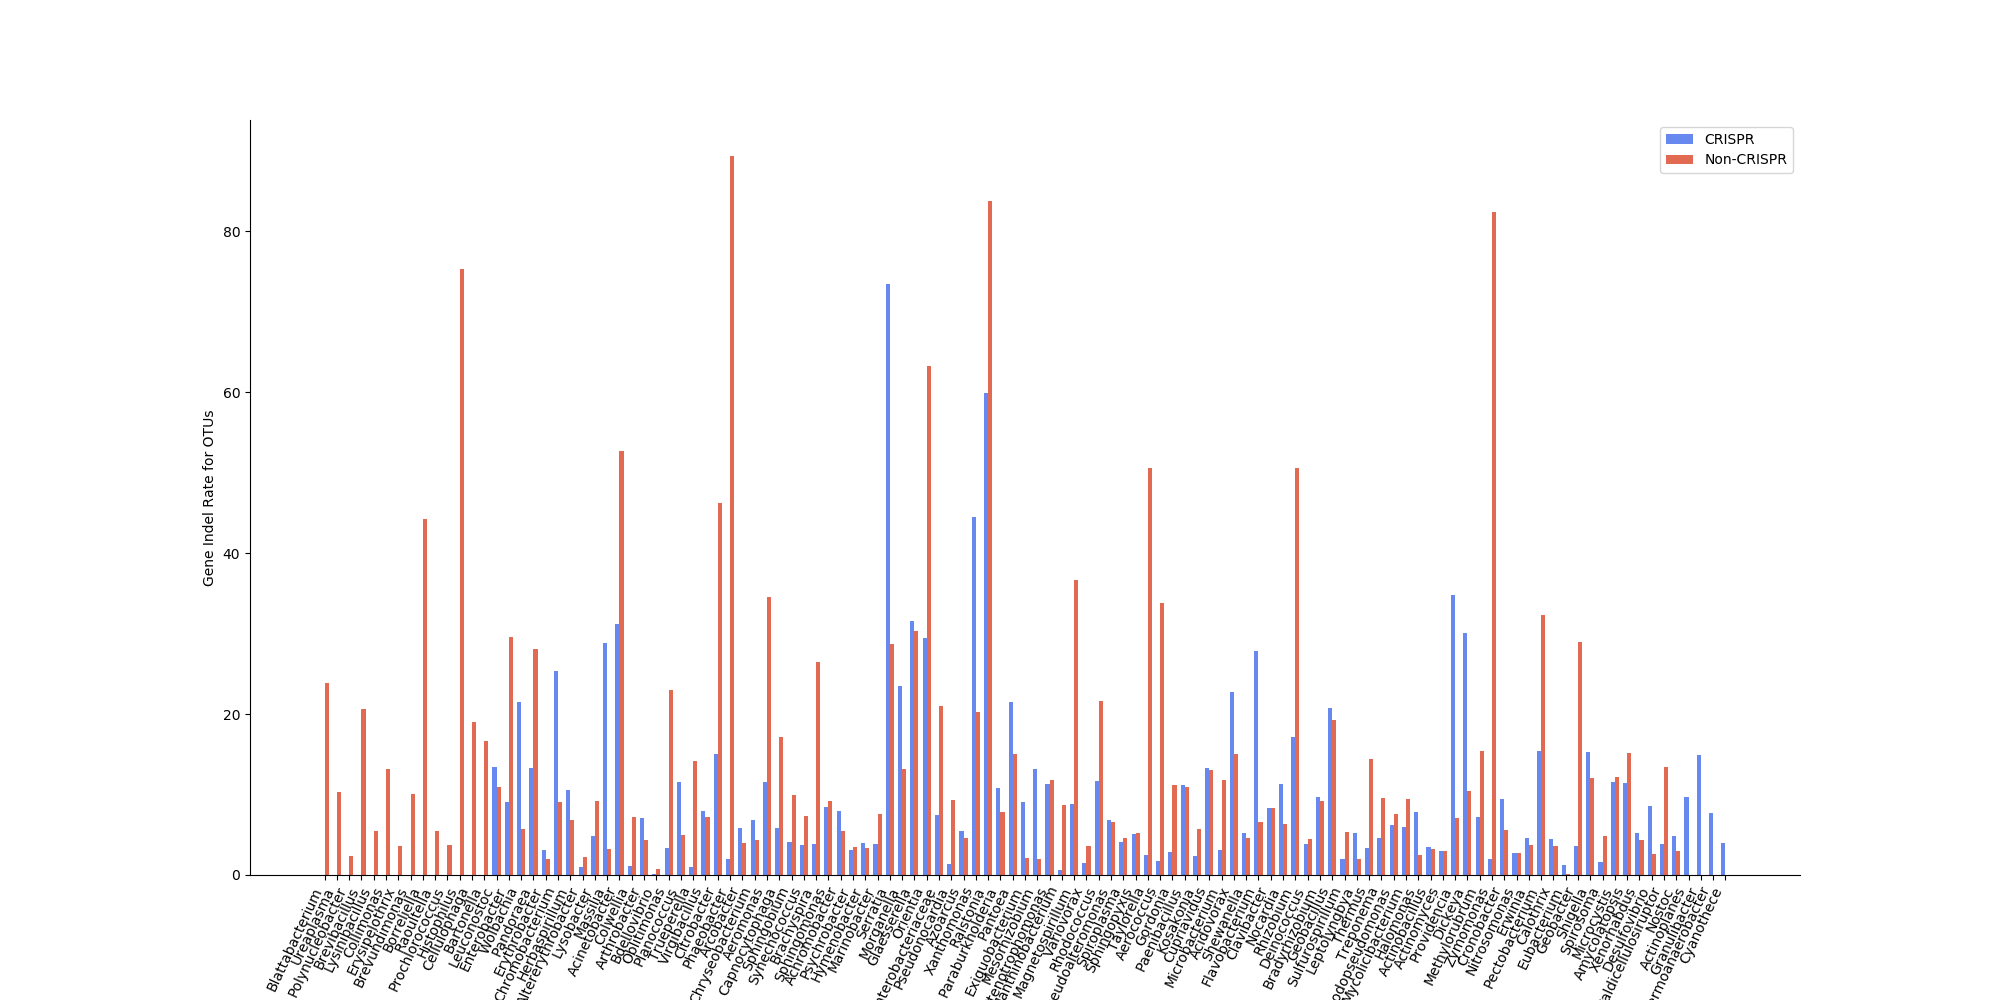
\includegraphics[width=1.2\linewidth]{c_nc_indel_bar.png}}
    \Put(175,325){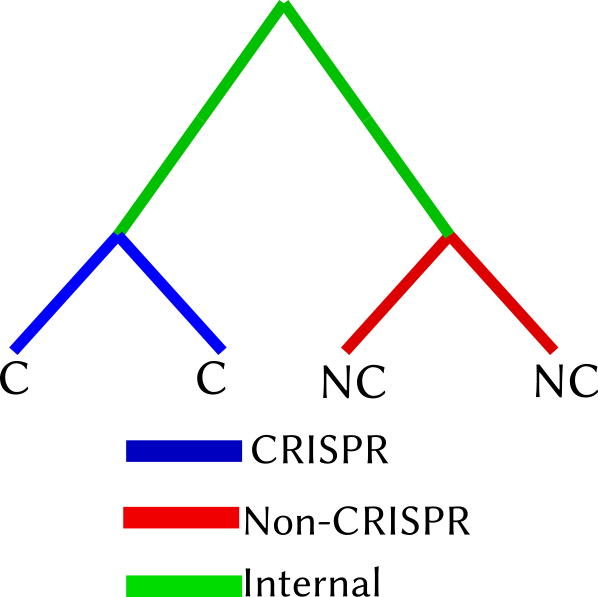
\includegraphics[width=0.2\linewidth]{partition_example.png}}
\end{frame}
\begin{frame}[fragile]{Gene Indel Rates}
    \makebox[\textwidth][c]{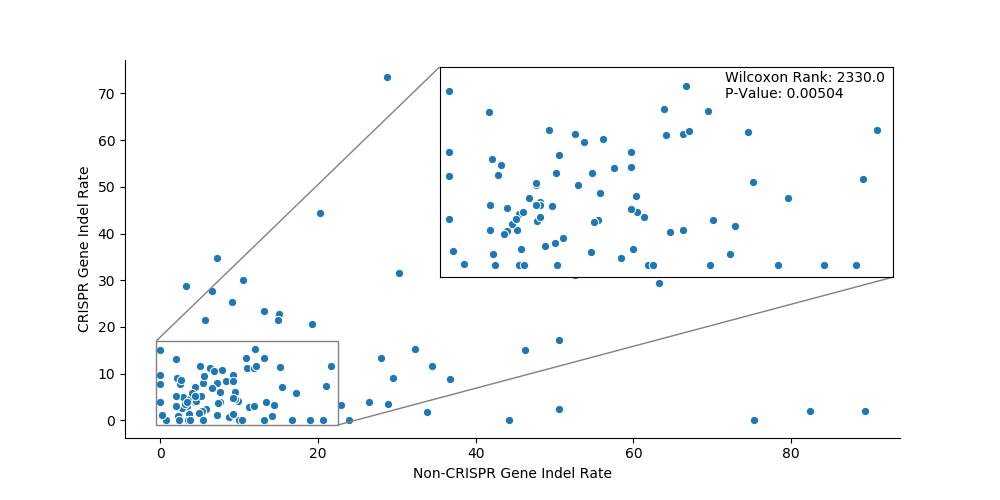
\includegraphics[width=1.2\linewidth]{c_nc_rate_scatter.png}}
    \Put(25,325){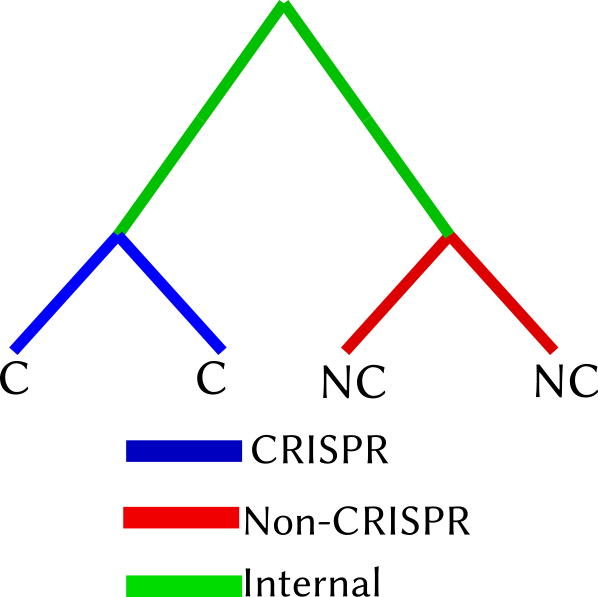
\includegraphics[width=0.2\linewidth]{partition_example.png}}
\end{frame}
\begin{frame}[fragile]{Gene Indel Rate Vs. Fraction of CRISPR OTUs}
    \makebox[\textwidth][c]{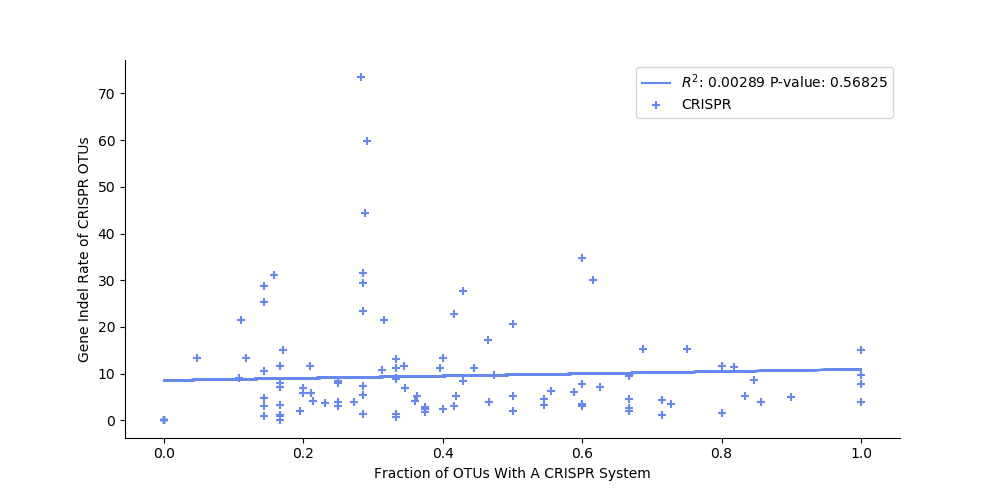
\includegraphics[width=1.25\linewidth]{crate_cfrac_scatter.png}}
    \Put(250,250){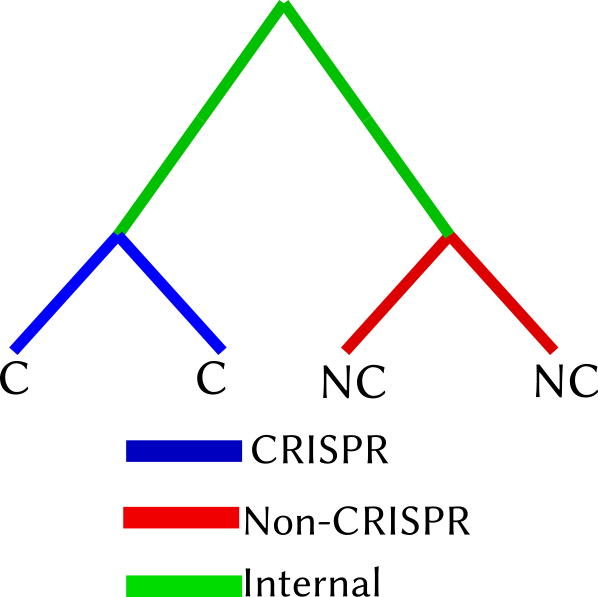
\includegraphics[width=0.2\linewidth]{partition_example.png}}
\end{frame}
\begin{frame}[fragile]{Gene Indel Rate Vs. Fraction of CRISPR OTUs}
    \makebox[\textwidth][c]{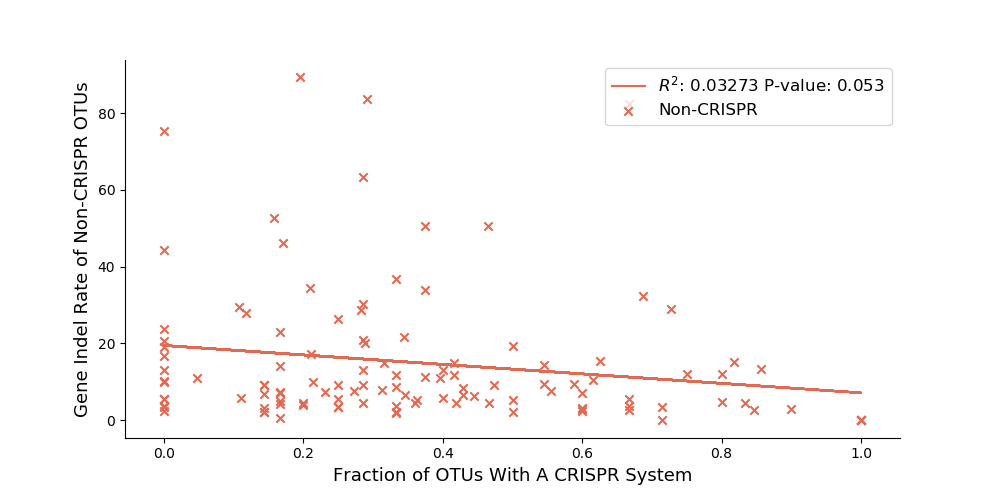
\includegraphics[width=1.25\linewidth]{ncrate_cfrac_scatter.png}}
    \Put(250,250){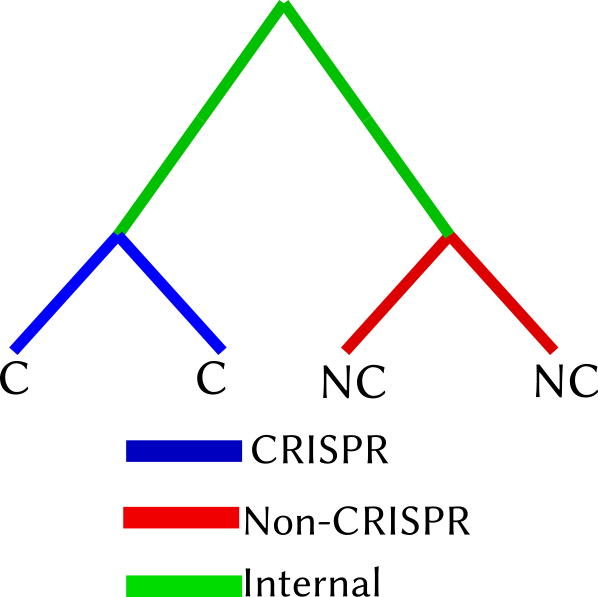
\includegraphics[width=0.2\linewidth]{partition_example.png}}
\end{frame}
\begin{frame}[fragile]{Mean Node Weighted Clustering Coefficient}
\begin{figure}[htb!]
    \makebox[\textwidth][c]{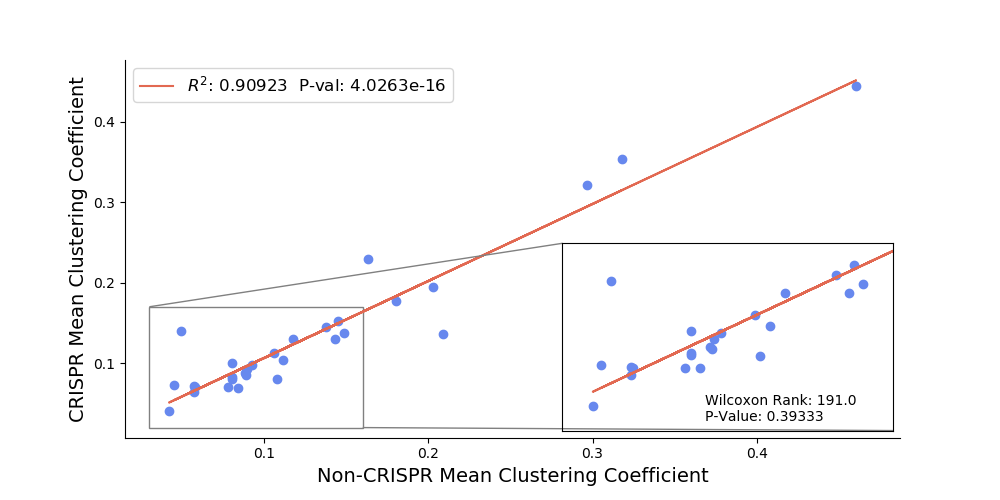
\includegraphics[width=1.2\linewidth]{c_nc_clust_scatter.png}}
\end{figure}
\end{frame}
\section{Conclusion}
\begin{frame}[fragile]{}%Conclusion}
    \begin{center}
        \Huge \textcolor{OliveGreen}{Conclusion}
    \end{center}
    \addtocounter{framenumber}{-1}
\end{frame}
\begin{frame}[fragile]{Findings}
    \begin{itemize}
        \item<2-> Large variation in \ac{hgt} rate between genera.
        \item<3-> \ac{crspc} systems broadly associated with lower \ac{hgt} rates, with prominent exceptions
        %\item<4-> High mixing between \ac{crsp} and non-\ac{crsp} \ac{otu}s
        \item<4-> Population level effects of \ac{crspc} systems may decrease \ac{hgt} rates
        \item<5-> Interplay of \ac{crspc} systems  and \ac{hgt} is complex and warrants further study
    \end{itemize}
\end{frame}
\begin{frame}[fragile]{Possible Future Directions}
\begin{itemize}
    \item<2-> \textbf{Intergenic comparisons}: Combine any set of fasta files from \ac{otu}s for analyzing transfer dynamics
    \item<3-> \textbf{Inferring direction}: Directed networks more available analytic tools than undirected networks ones
    \item<4-> \textbf{Continuous \ac{crsp} activity}: Labeling nodes by estimated \ac{crsp} activity (array length, transciptomic data, etc.)
    \item<5-> \textbf{Considering bacterial ecology and environments}: Consider geographically close \ac{otu}s or differences between networks due to environmental factors
    \item<6-> \textbf{Gene function analysis}: Considering the transfer dynamics of different functional classes of genes
    \item<7-> \textbf{Studying movement of \ac{crsp} systems}: Studying how frequently \ac{crsp} systems themselves are transferred from arrays, \textit{Cas} genes
\end{itemize}
\end{frame}
\begin{frame}[fragile]{}%Is Sharing Caring?}
    \begin{center}
        \onslide<1-> \Huge \textcolor{OliveGreen}{Is Sharing Caring?}\\
        \vspace{0.2in}
        \Large
        \onslide<2-> Yes, for researchers\\
        \onslide<3-> Jury's still out for bacteria
    \end{center}
\end{frame}
\begin{frame}[fragile]{Thanks}
    \begin{multicols}{2}
    %Names
    \begin{minipage}[b][40ex][t]{\linewidth}
    Thank you to
    \begin{itemize}
        \item Dr. G. Brian Golding
        \item Dr. Ben Evans
        \item The Golding lab
            \begin{itemize}
                \item Caitlin Simopoulos
                \item Daniella Lato
                \item Zachery Dickson
                \item Sam Long
                \item George Long
                \item Lucy Zhang
                \item Brianne Laverty
                \item Nicole Zhang
            \end{itemize}
        \item Everyone here for listening
    \end{itemize}
    \end{minipage}
    %mcmaster logo
    \begin{minipage}[b][20ex][t]{\linewidth}
    \begin{figure}[htb!]
        \makebox[\textwidth][c]{
\includegraphics[width=\linewidth]{mcmaster_logo.png}}
    \end{figure}
    \end{minipage}
    %Github link
    \begin{minipage}[b][20ex][t]{\linewidth}
        \vspace{0.1in}
        All code used for this project is available at
        \myurl[blue]{https://github.com/DJSiddharthVader/thesis_SidReed}
    \end{minipage}
    \end{multicols}
\end{frame}
\backupbegin
\section*{Backup Slides}
% Background
\begin{frame}[fragile]{CRISPR Cost Complexity and Curbing It (Expanded)}
    \begin{columns}
    \begin{column}{0.5\textwidth} %Costs
        \begin{itemize}
        \item Cost trade off factors:
        \begin{itemize}
            \item Metabolic maintenance \autocite{crispgen}
            \item Off-target effects (autoimmune) \autocite{selfcrisp}
            \item Environmental pressures \autocite{hospital}
            \item Phage virulence/density \autocite{acqorres}
            \item Anti-CRISPR systems \autocite{acqorres}
            \item Prophage abundance \autocite{transhgt}
        \end{itemize}
        \end{itemize}
    \end{column}
    \begin{column}{0.5\textwidth} %Curbing it
    \begin{itemize}
        \item Cost Reduction Strategies
        \begin{itemize}
            \item Selective CRISPR inactivation \autocite{crispgen}
            \item CRISPRs themselves can be transferred $\implies$ population level immunity \autocite{crisprlgt}
            \item CRISPR can enhance transduction-mediated HGT \autocite{transhgt}
        \end{itemize}
    \end{itemize}
    \end{column}
    \end{columns}
\end{frame}
\begin{frame}[fragile]{Rate Influencing Factors}
    \begin{itemize}
        \item Amount of exogenous DNA/cell density/phage density
        \item Selective pressures
        \item Metabolic costs
        \item Sequence compatibility
    \end{itemize}
\end{frame}
\begin{frame}[fragile]{Pan-Genomes}
    \begin{columns}
    \begin{column}{0.5\textwidth}
        \begin{figure}[htb!]
            \makebox[\textwidth][c]{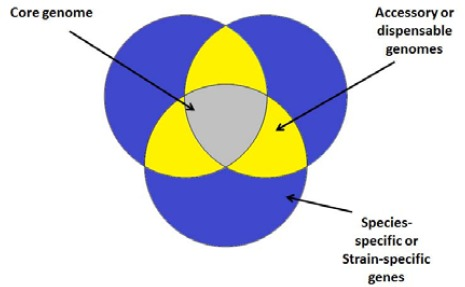
\includegraphics[width=\linewidth]{pangenome_pang.jpg}}
            \autocite{pang}
        \end{figure}
    \end{column}
    \begin{column}{0.5\textwidth}
        \begin{figure}[htb!]
            \makebox[\textwidth][c]{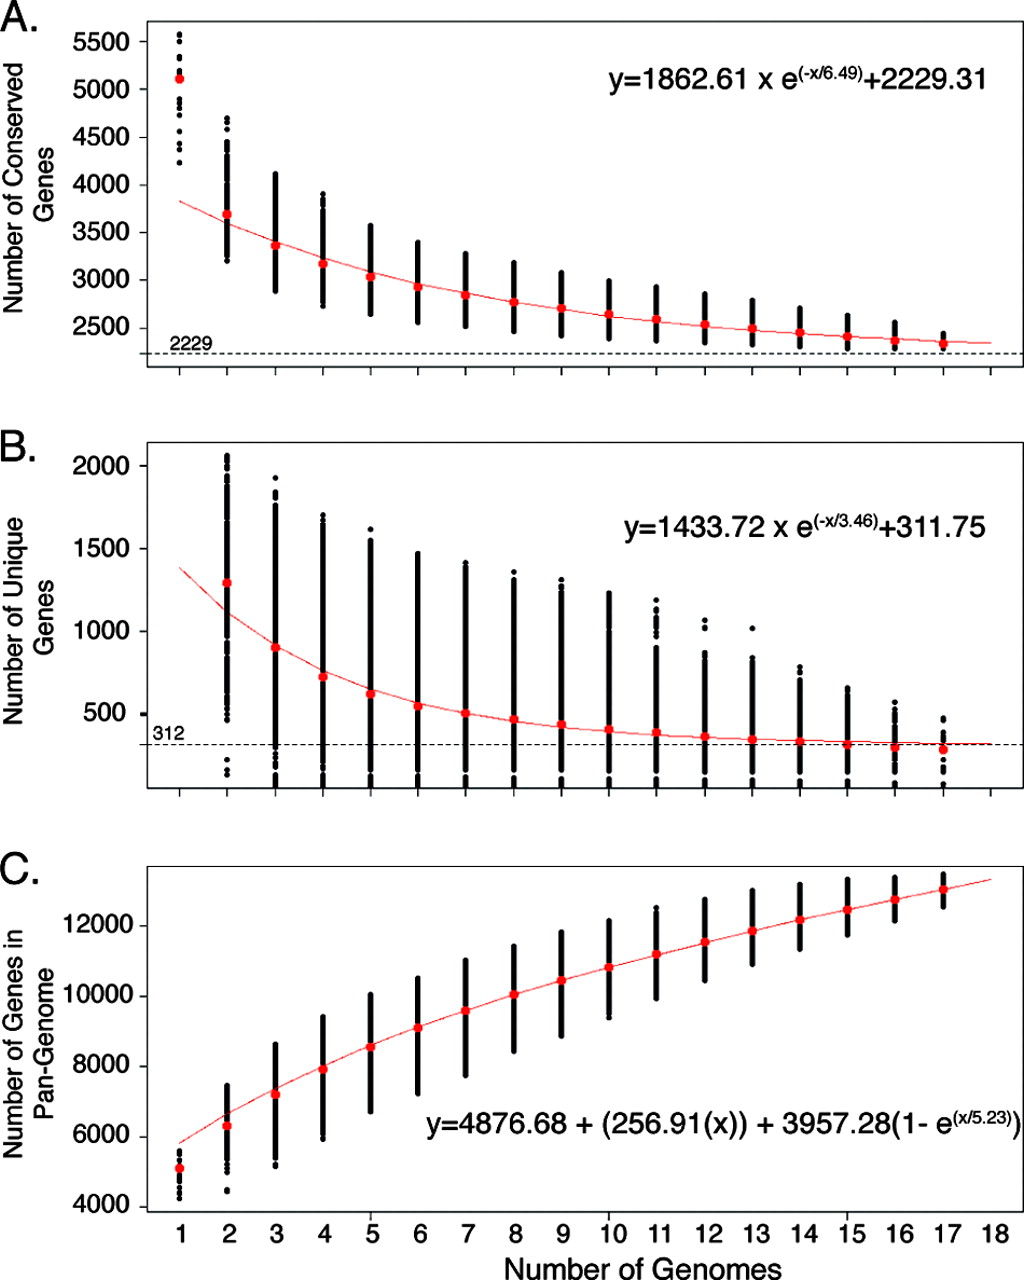
\includegraphics[width=0.8\linewidth]{pangGrapgs_ecopan.jpg}}
            \autocite{ecopan}
        \end{figure}
    \end{column}
    \end{columns}
\end{frame}
\begin{frame}[fragile]{HGT Applications}
    \begin{figure}[htb!]
        \makebox[\textwidth][c]{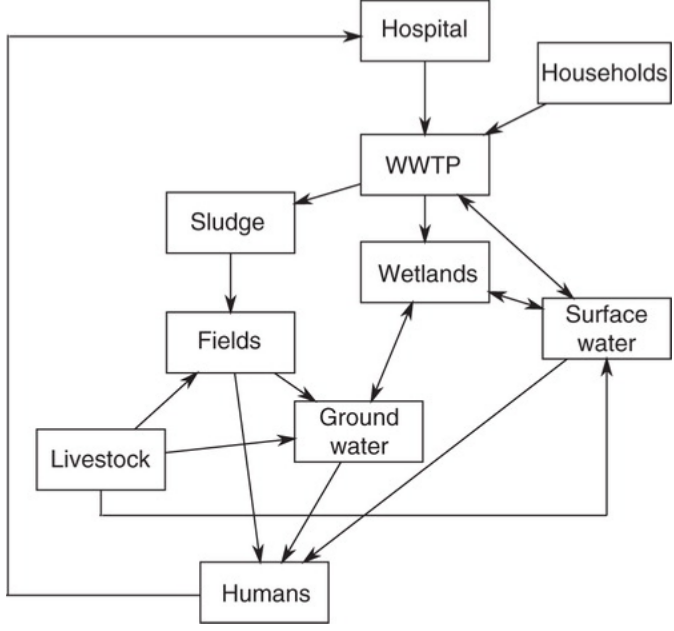
\includegraphics[width=0.6\linewidth]{spreadDiagram_argspread.png}}
        \autocite{argspread}
    \end{figure}
\end{frame}
\begin{frame}[fragile]{Prokaryotic ``Net of Life''}
    \begin{figure}[htb!]
        \makebox[\textwidth][c]{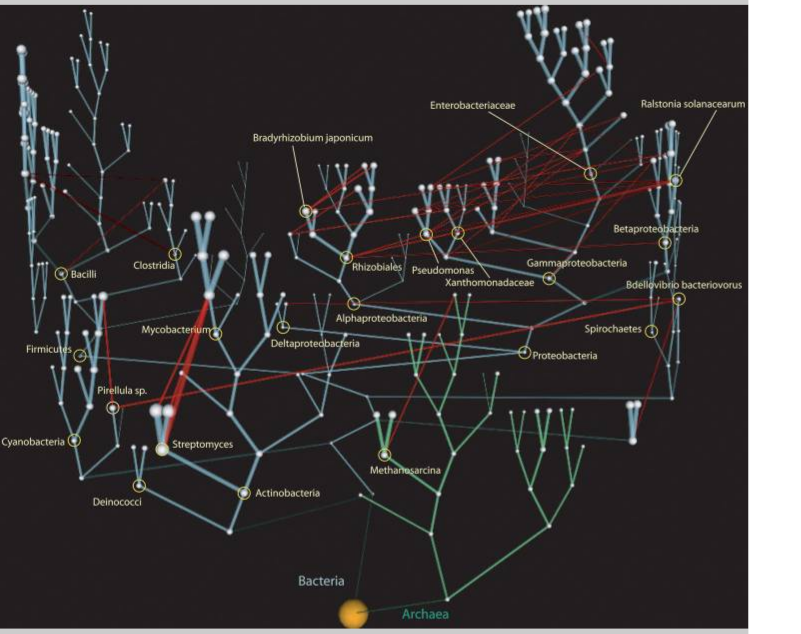
\includegraphics[width=0.7\linewidth]{net_netoflife.png}}
        \autocite{netoflife}
    \end{figure}
\end{frame}
% Methods
\begin{frame}[fragile]{Branch Partition Example}
    \begin{figure}[htb!]
        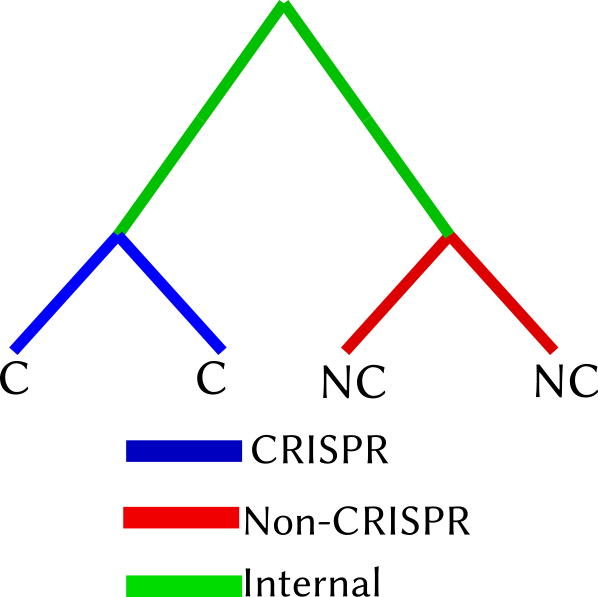
\includegraphics[width=0.5\linewidth]{partition_example.png}
    \end{figure}
\end{frame}
\begin{frame}[fragile]{Network Sampling}
    \begin{figure}[htb!]
        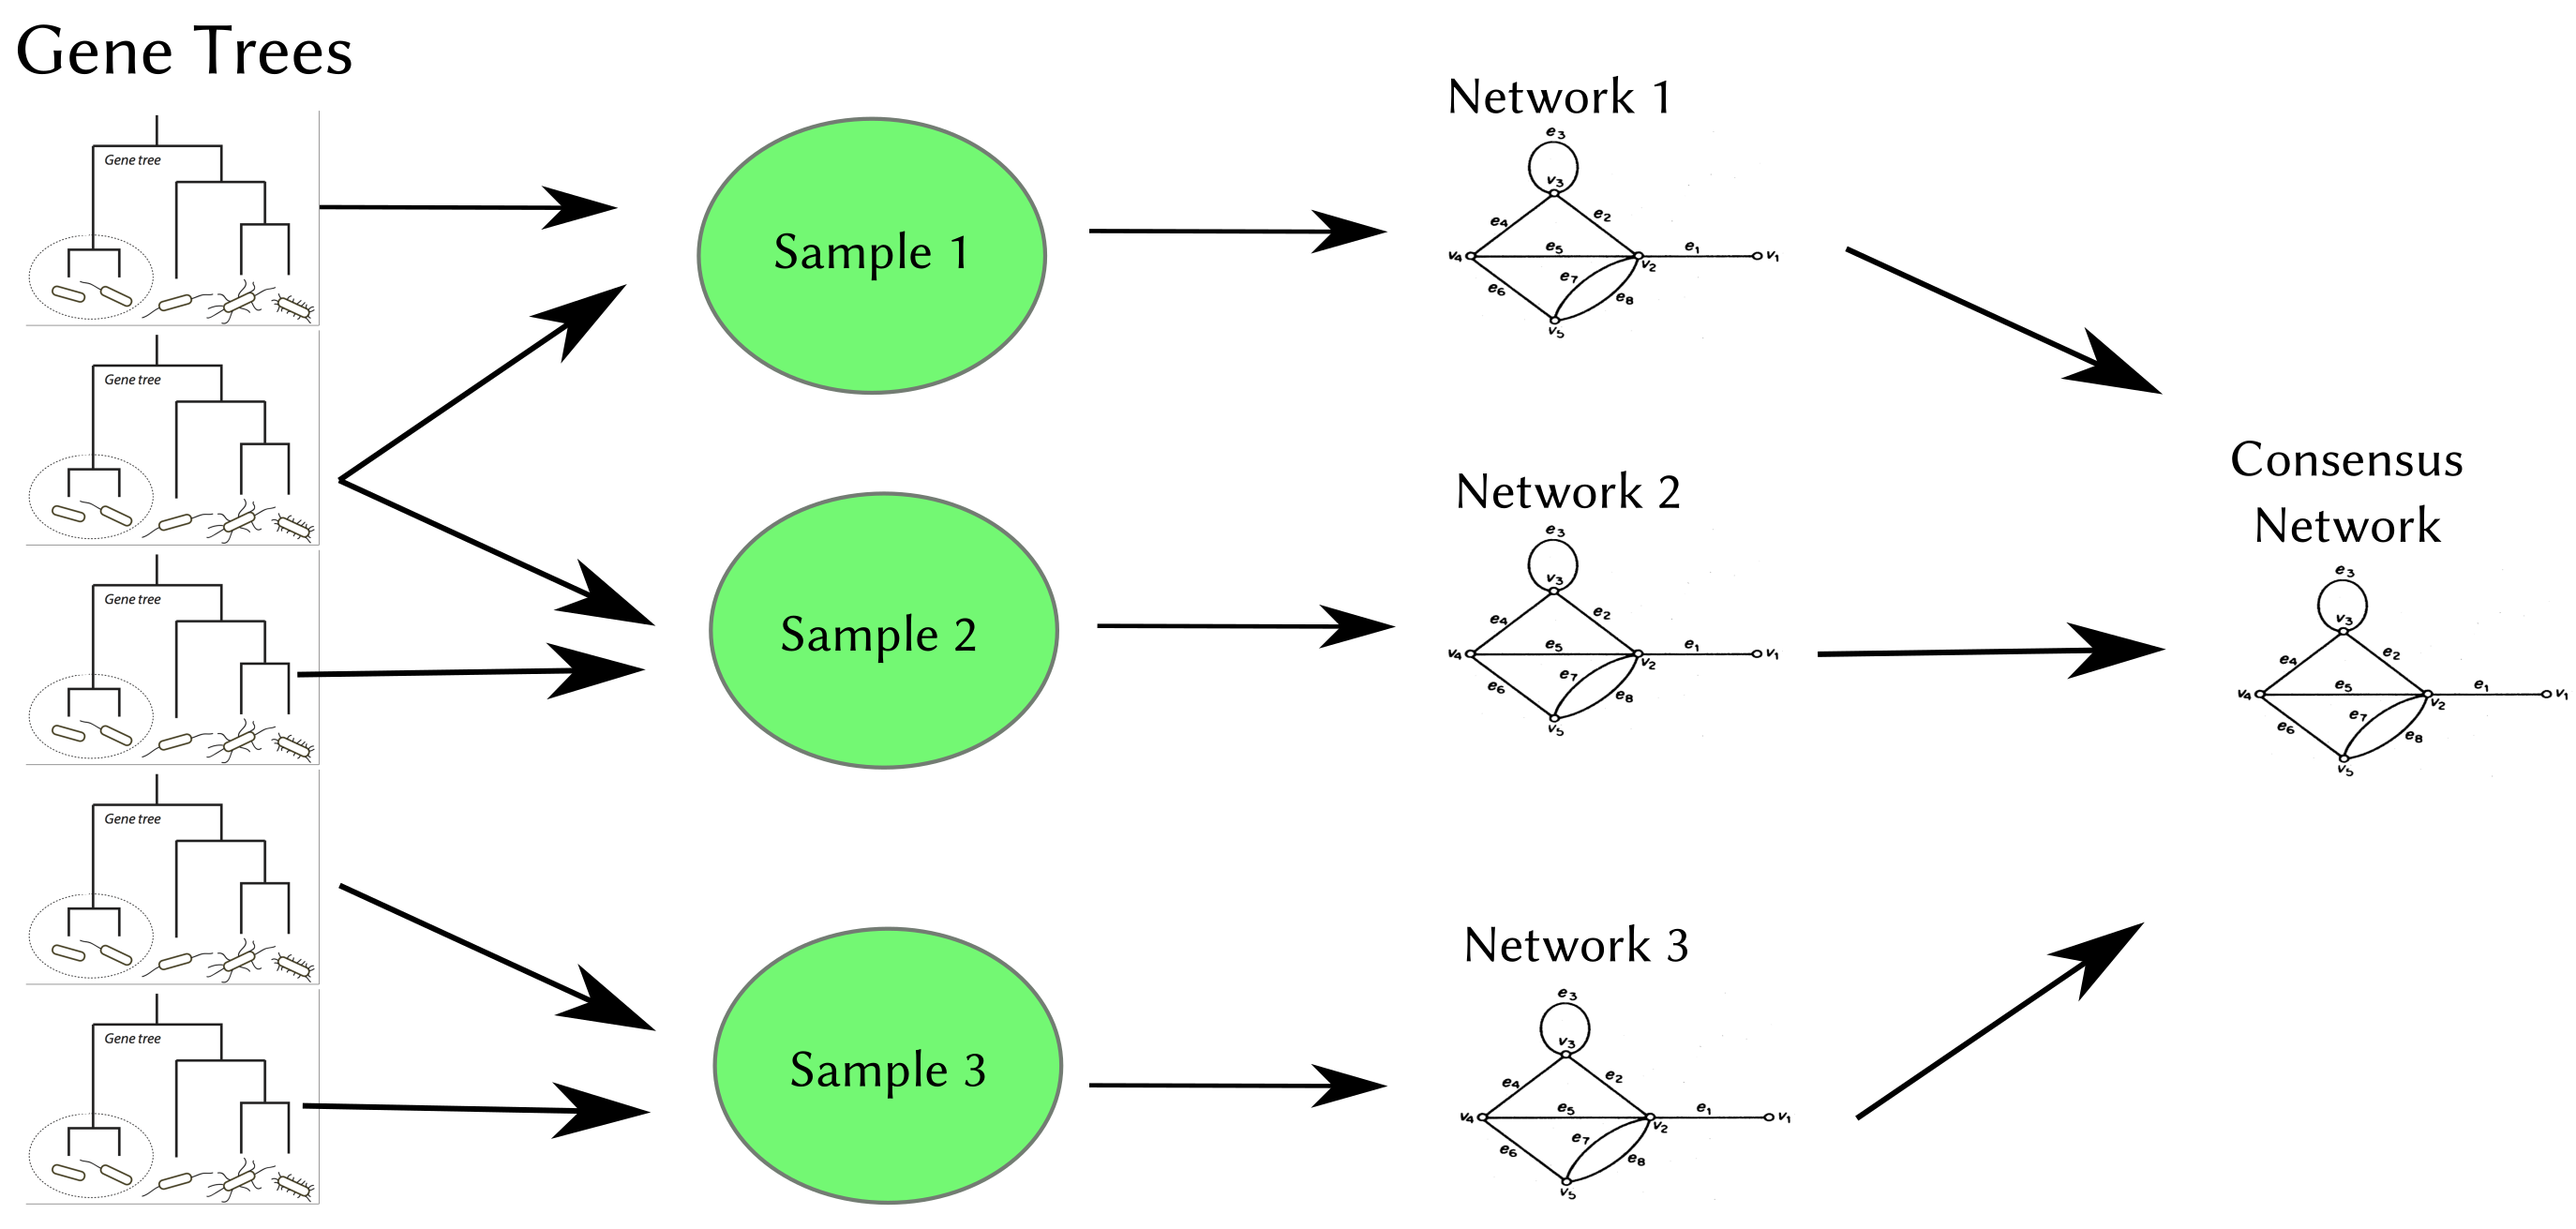
\includegraphics[width=\linewidth]{netsample.png}
    \end{figure}
\end{frame}
\begin{frame}[fragile]{CRISPR One Database Entry}
    \begin{figure}[htb!]
        \makebox[\textwidth][c]{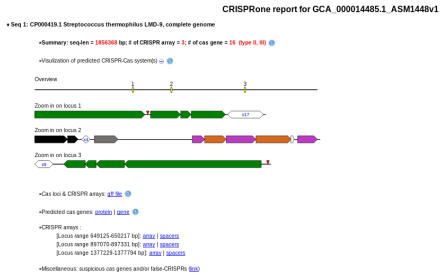
\includegraphics[width=0.8\linewidth]{CRISPROneEntry.png}}
    \end{figure}
\end{frame}
\begin{frame}[fragile]{Network Statistics}
    \begin{itemize}
        \item \textbf{Average Node Degree}: $\frac{1}{|N_u|}\sum_{uv}^{N_u} w_{uv}$ where $N_u$ is the set of nodes incident to $u$
        \item \textbf{Node Clustering Coefficient}:$\frac{1}{k_u(k_u-1)} \sum_{vw}^{T(u)} (\hat{w}_{uw} \hat{w}_{vw} \hat{w}_{uv})^{\frac{1}{3}}$ where $T(u)$ is the set of triangles containing $u$ \autocite{clustering}
        \item \textbf{Node Assortativity}: $A = \frac{Tr(M)-||M^2||}{1-||M^2||}$ Where $M$ is the mixing matrix of a given attribute and $||M||$ is the sum of all elements of $M$. $A \in [-1,1]$. \autocite{newmanmix}
        \item \textbf{Network Modularity}: $Q=\frac{1}{2m}\sum_{uv}^W [W_{uv} - \frac{k_u k_v}{2m}]\delta(u,v)$ where $m$ is the total weight of alledges, $k_u$ is the degree of $u$ and $\delta(u,v)$ is 1 if $u$ and $v$ both have or do not have \ac{crsp} systems and 0 otherwise. $Q \in [-1,1]$ \autocite{modularity}
        %\item \textbf{Average Edge Weight}: $\frac{1}{N_c}\sum_i w_i$, The average edge weight for all nodes with \ac{crsp} or without \ac{crsp}
        %\item \textbf{Node Eigenvector Centrality}: $\frac{N-1}{\sum_v d(u,v)}$ where $d(x,y)$ is the length of the shortest path $v \to u$. \autocite{egcen}
%        \item \textbf{Edge Weight KL Divergence}: $D_{KL}(P||Q)= \int_{-\infty}^{\infty} p(x)log(\frac{p(x)}{q(x)})dx$
%        \item \textbf{Network Diameter}: Shortest path between the 2 furthest nodes.
%        \item \textbf{Network Density}: $\frac{2E}{N(N-1)}$
    \end{itemize}
\end{frame}
\begin{frame}[fragile]{Phylogenomic Network Construction}
    \begin{figure}[htb!]
        \makebox[\textwidth][c]{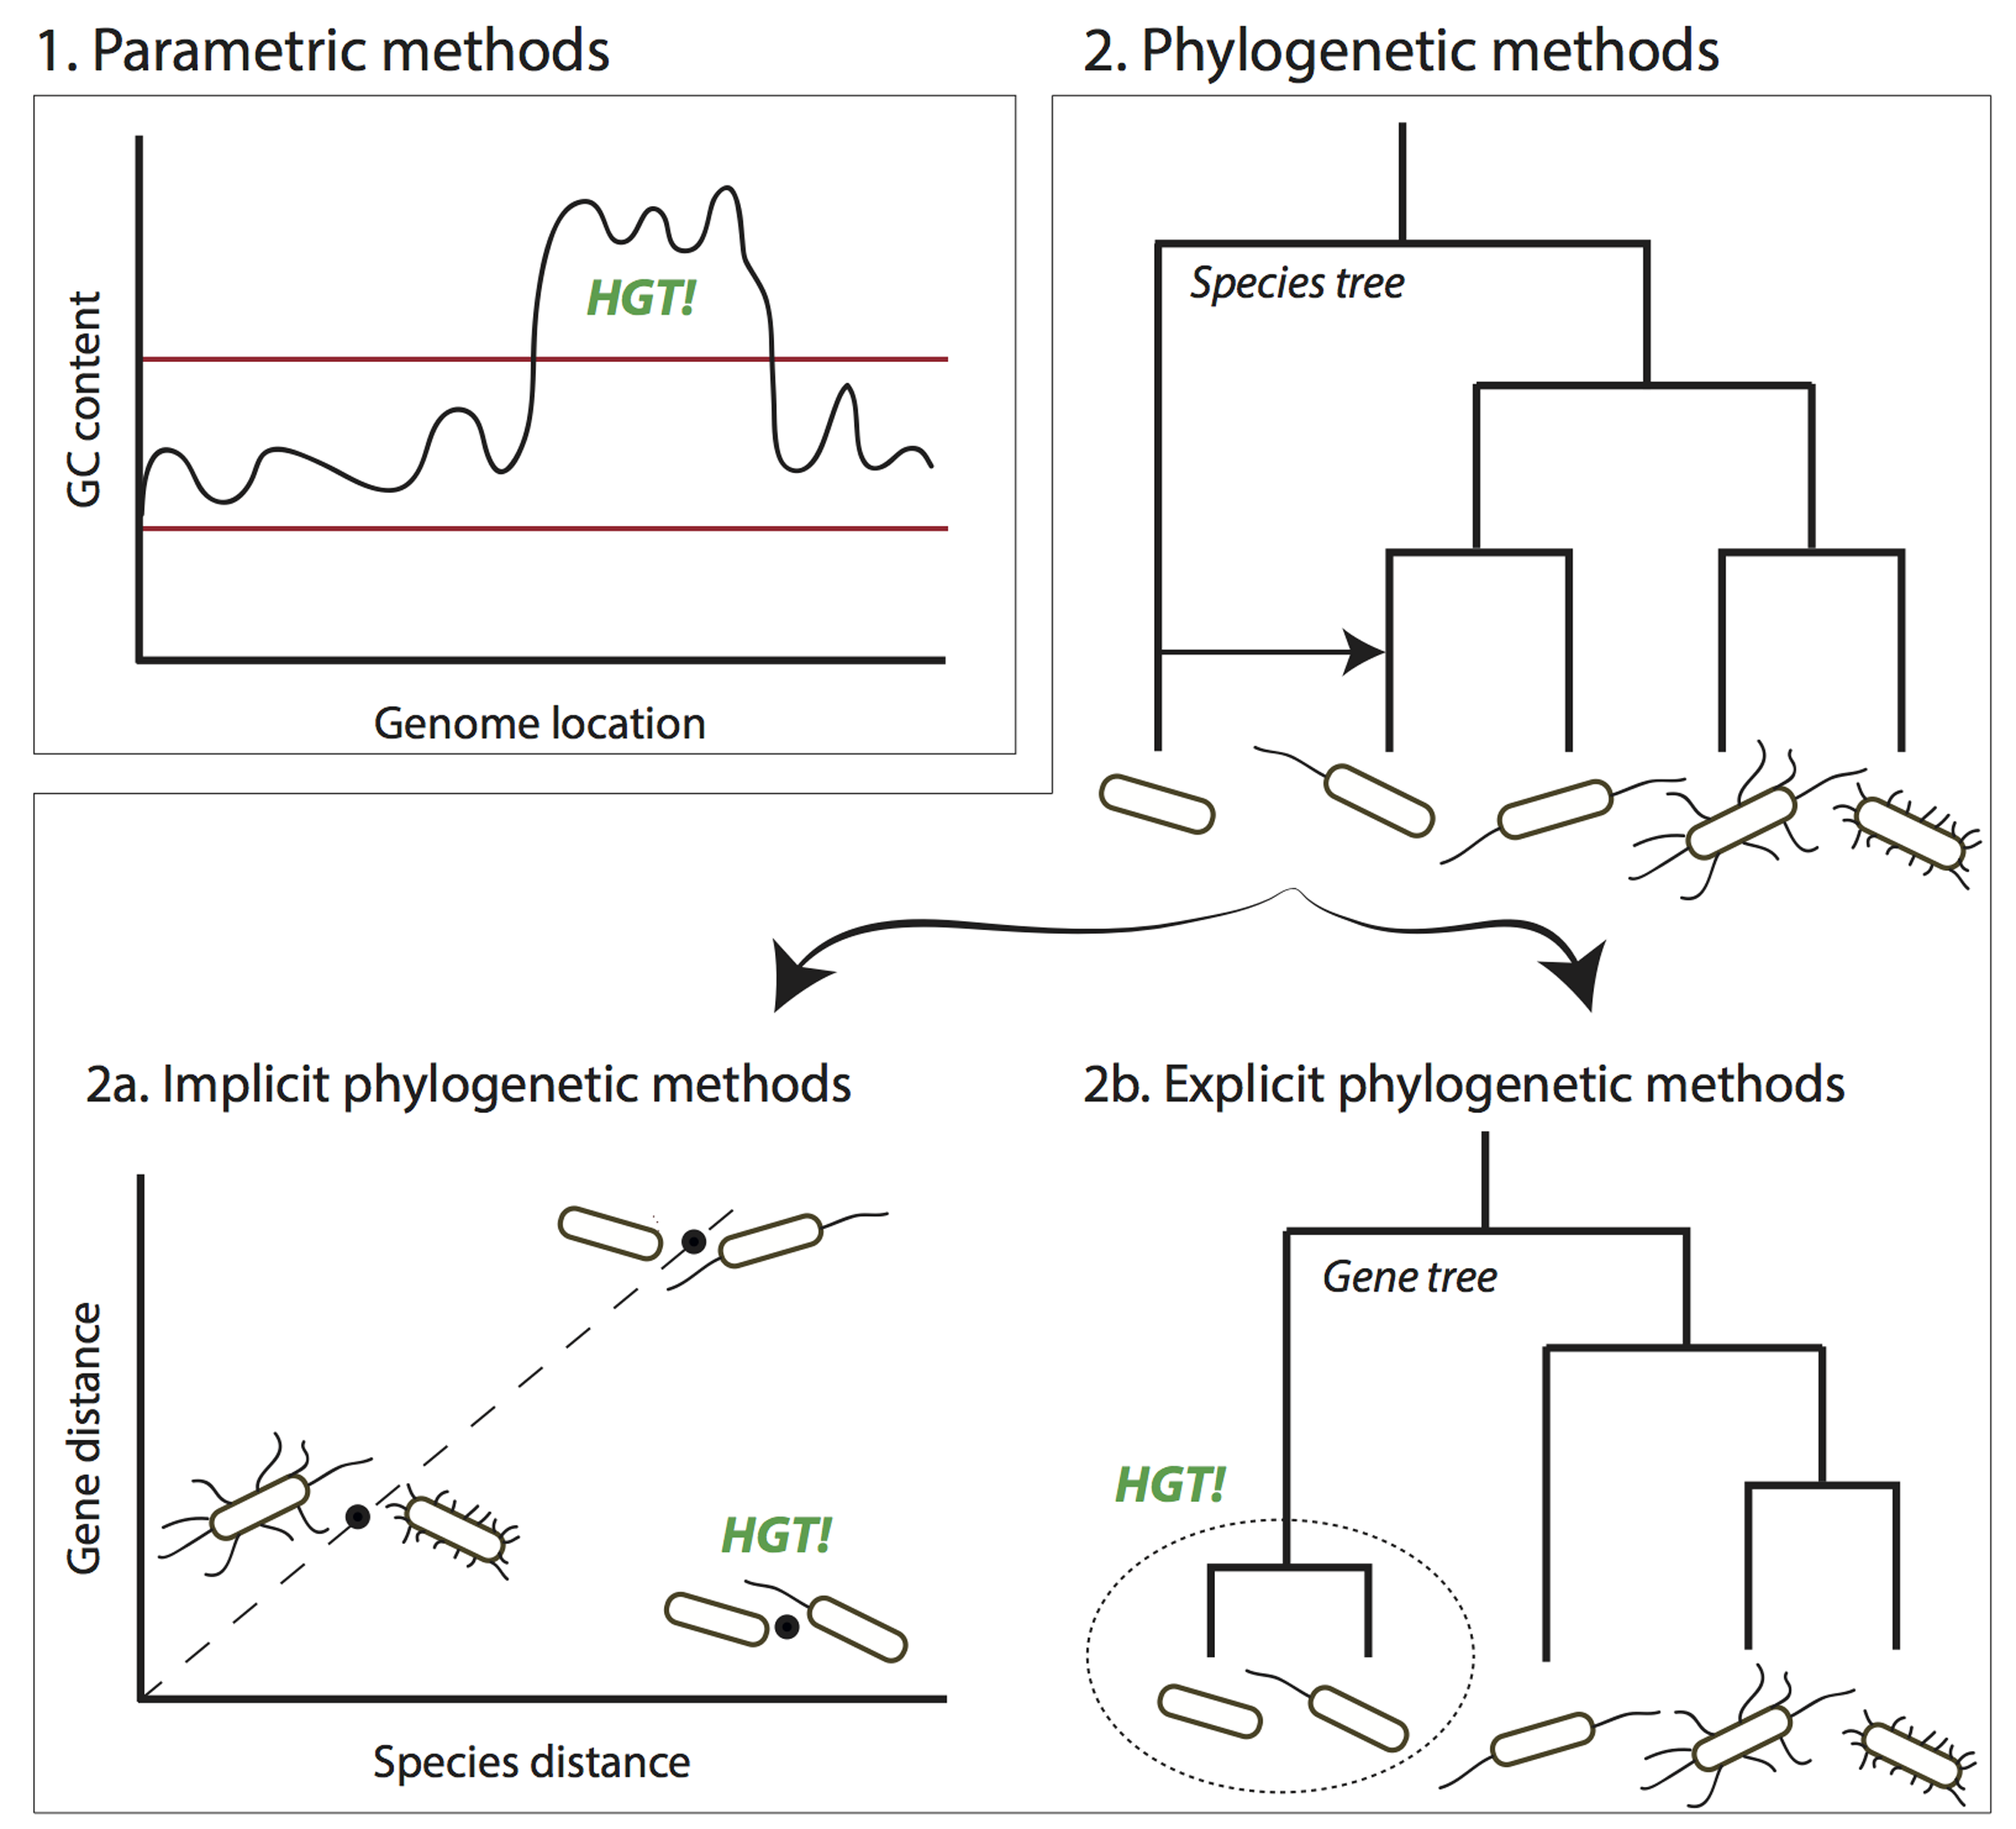
\includegraphics[width=0.6\linewidth]{hgtiInferenceMethods_ihgt.png}}
        \autocite{ihgt}
    \end{figure}
\end{frame}
% Results
\begin{frame}[fragile]{Genus Size Distribution}
    \makebox[\textwidth][c]{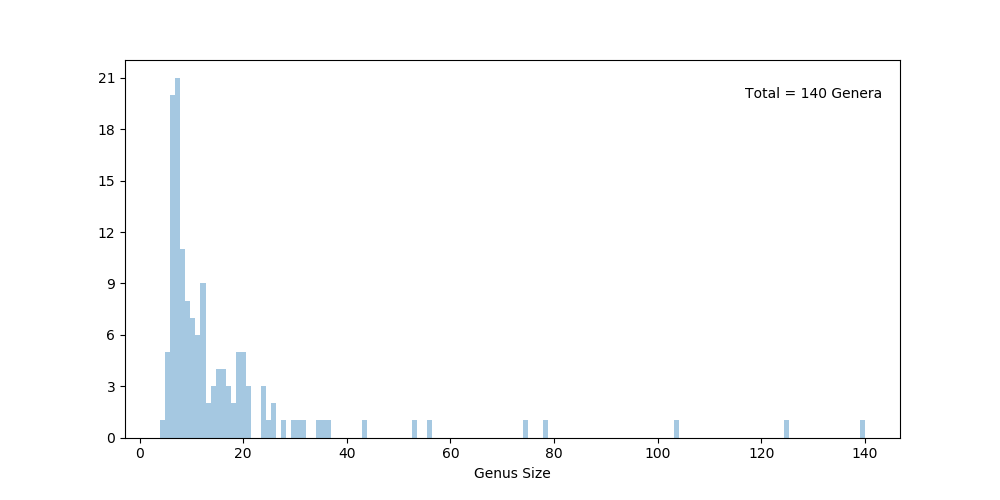
\includegraphics[width=1.2\linewidth]{genus_size_dist.png}}
\end{frame}
\begin{frame}[fragile]{Sphingomonas Species Tree}
    \makebox[\textwidth][c]{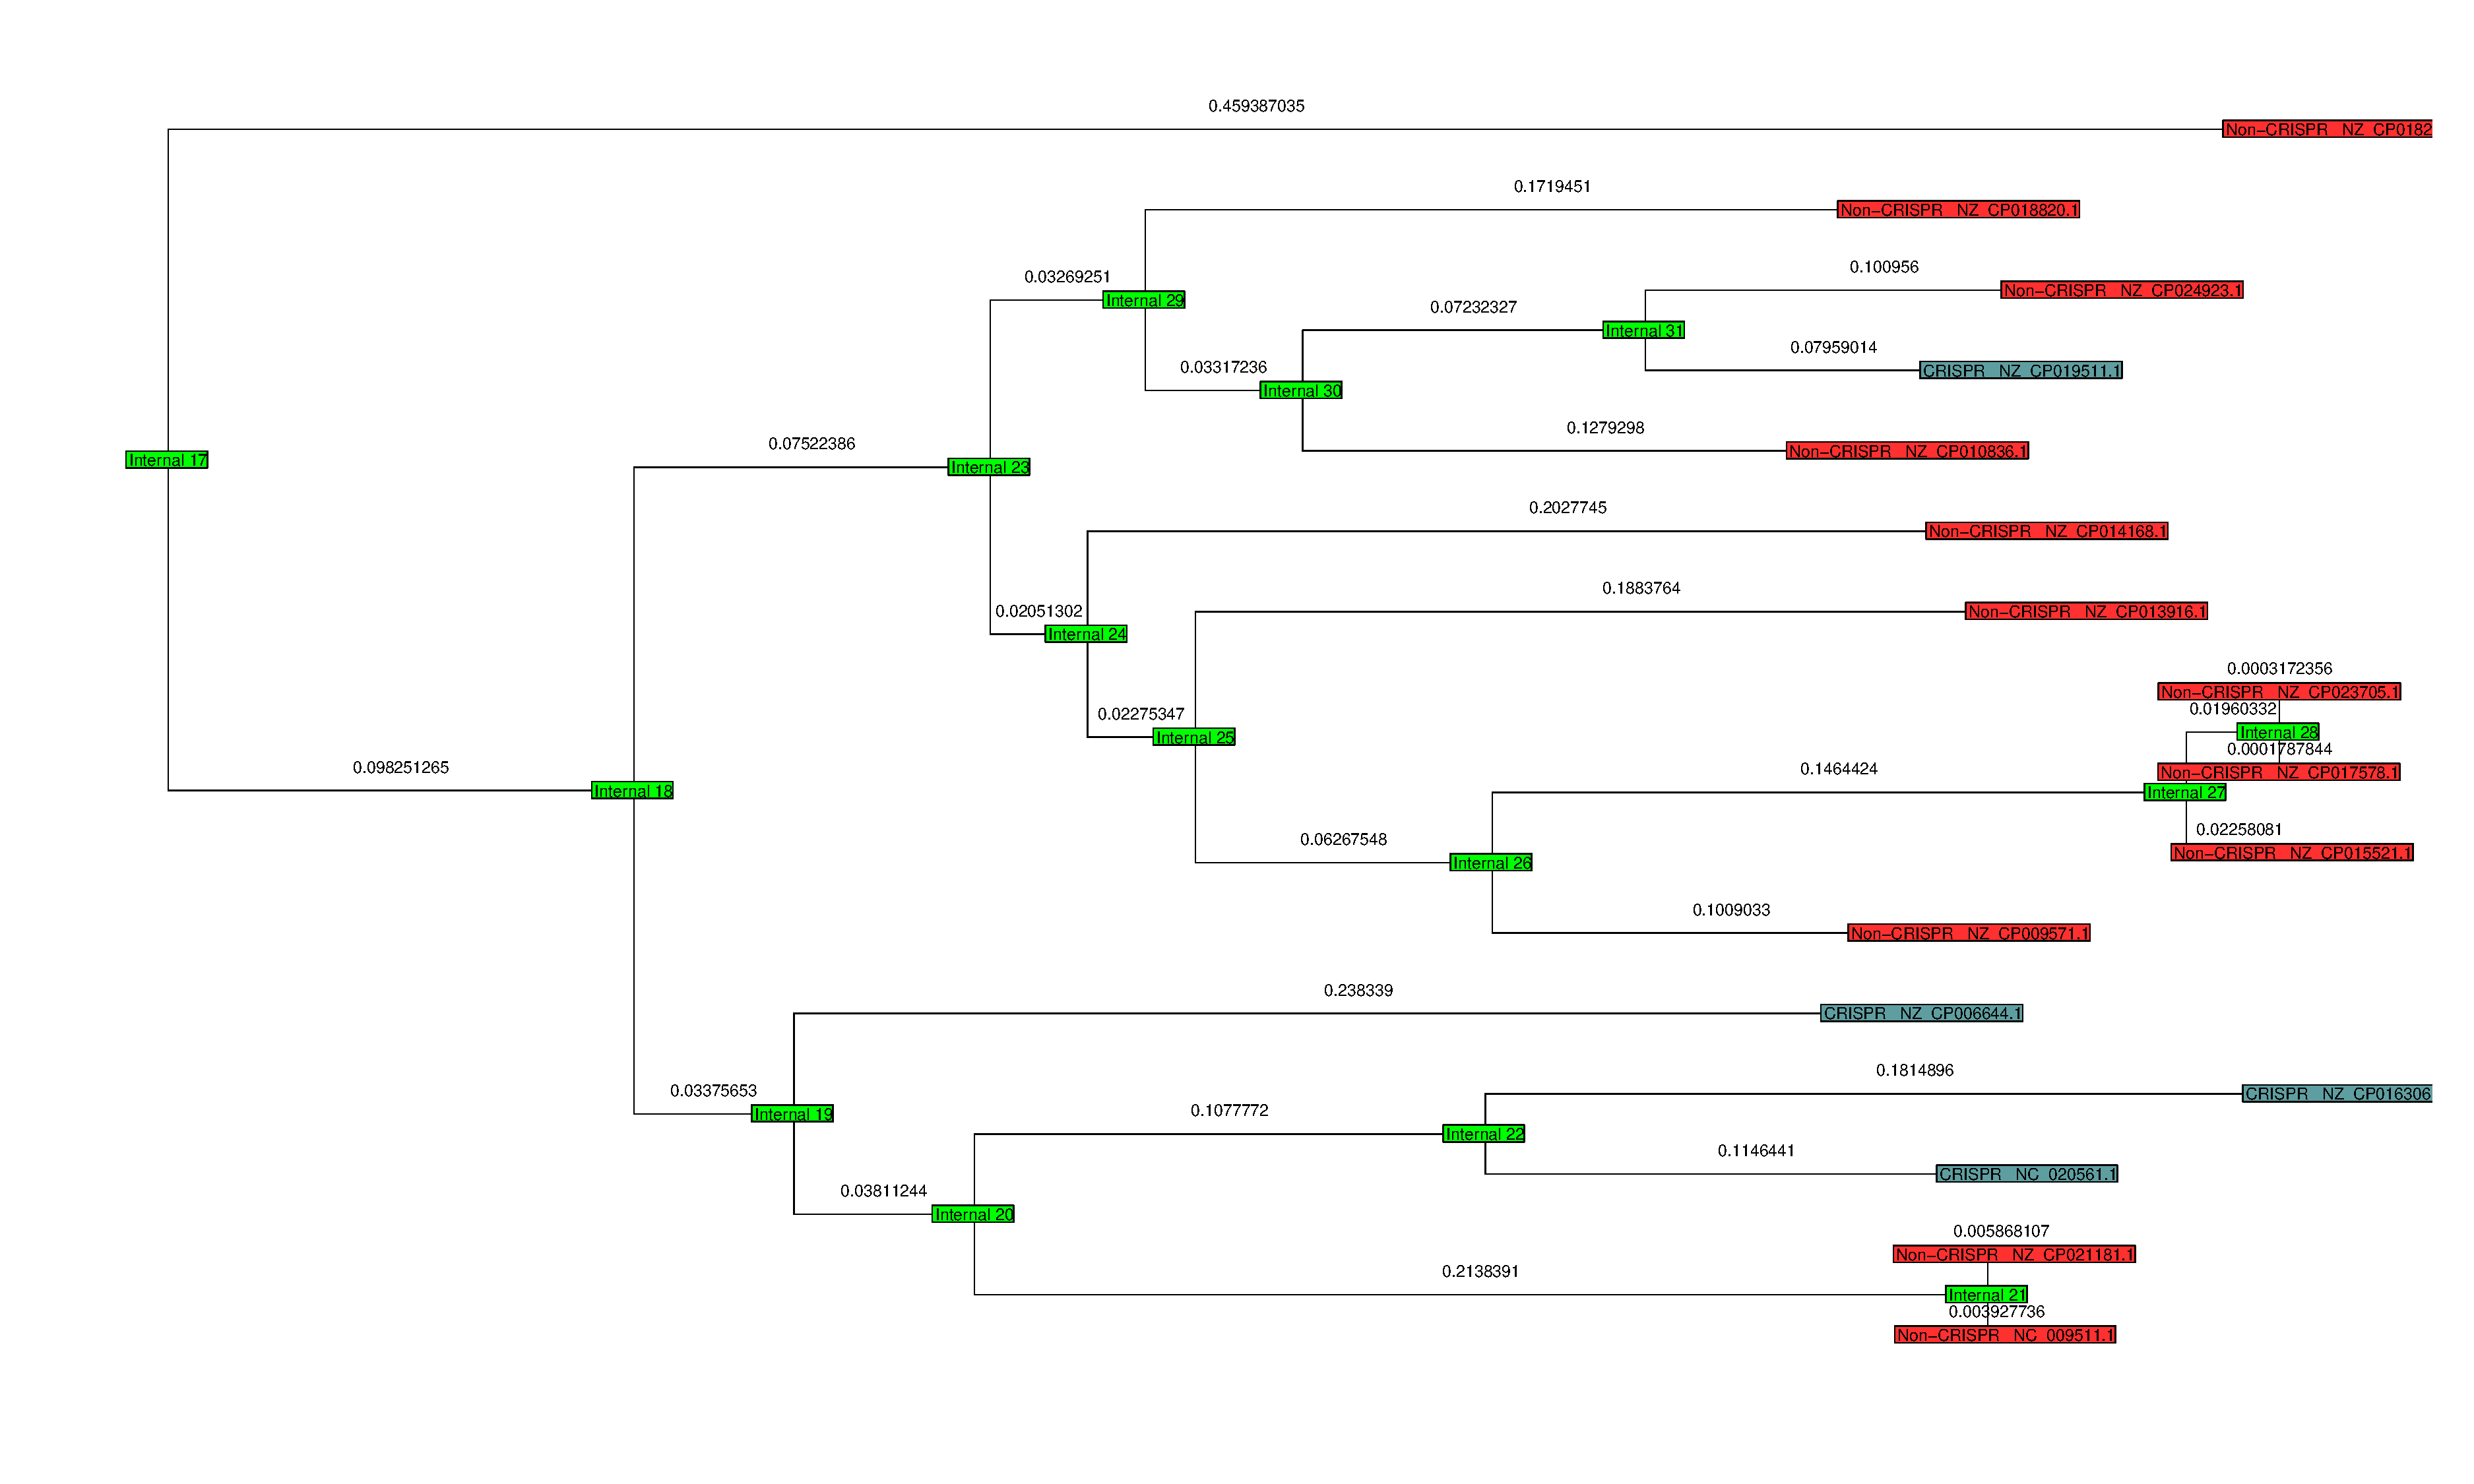
\includegraphics[width=\linewidth]{../nontext/figures/Sphingomonas_labelled_cladogram.pdf}}
\end{frame}
% Extras
\begin{frame}[fragile]{Assortativity Distributions}
    \begin{figure}[htb!]
        \makebox[\textwidth][c]{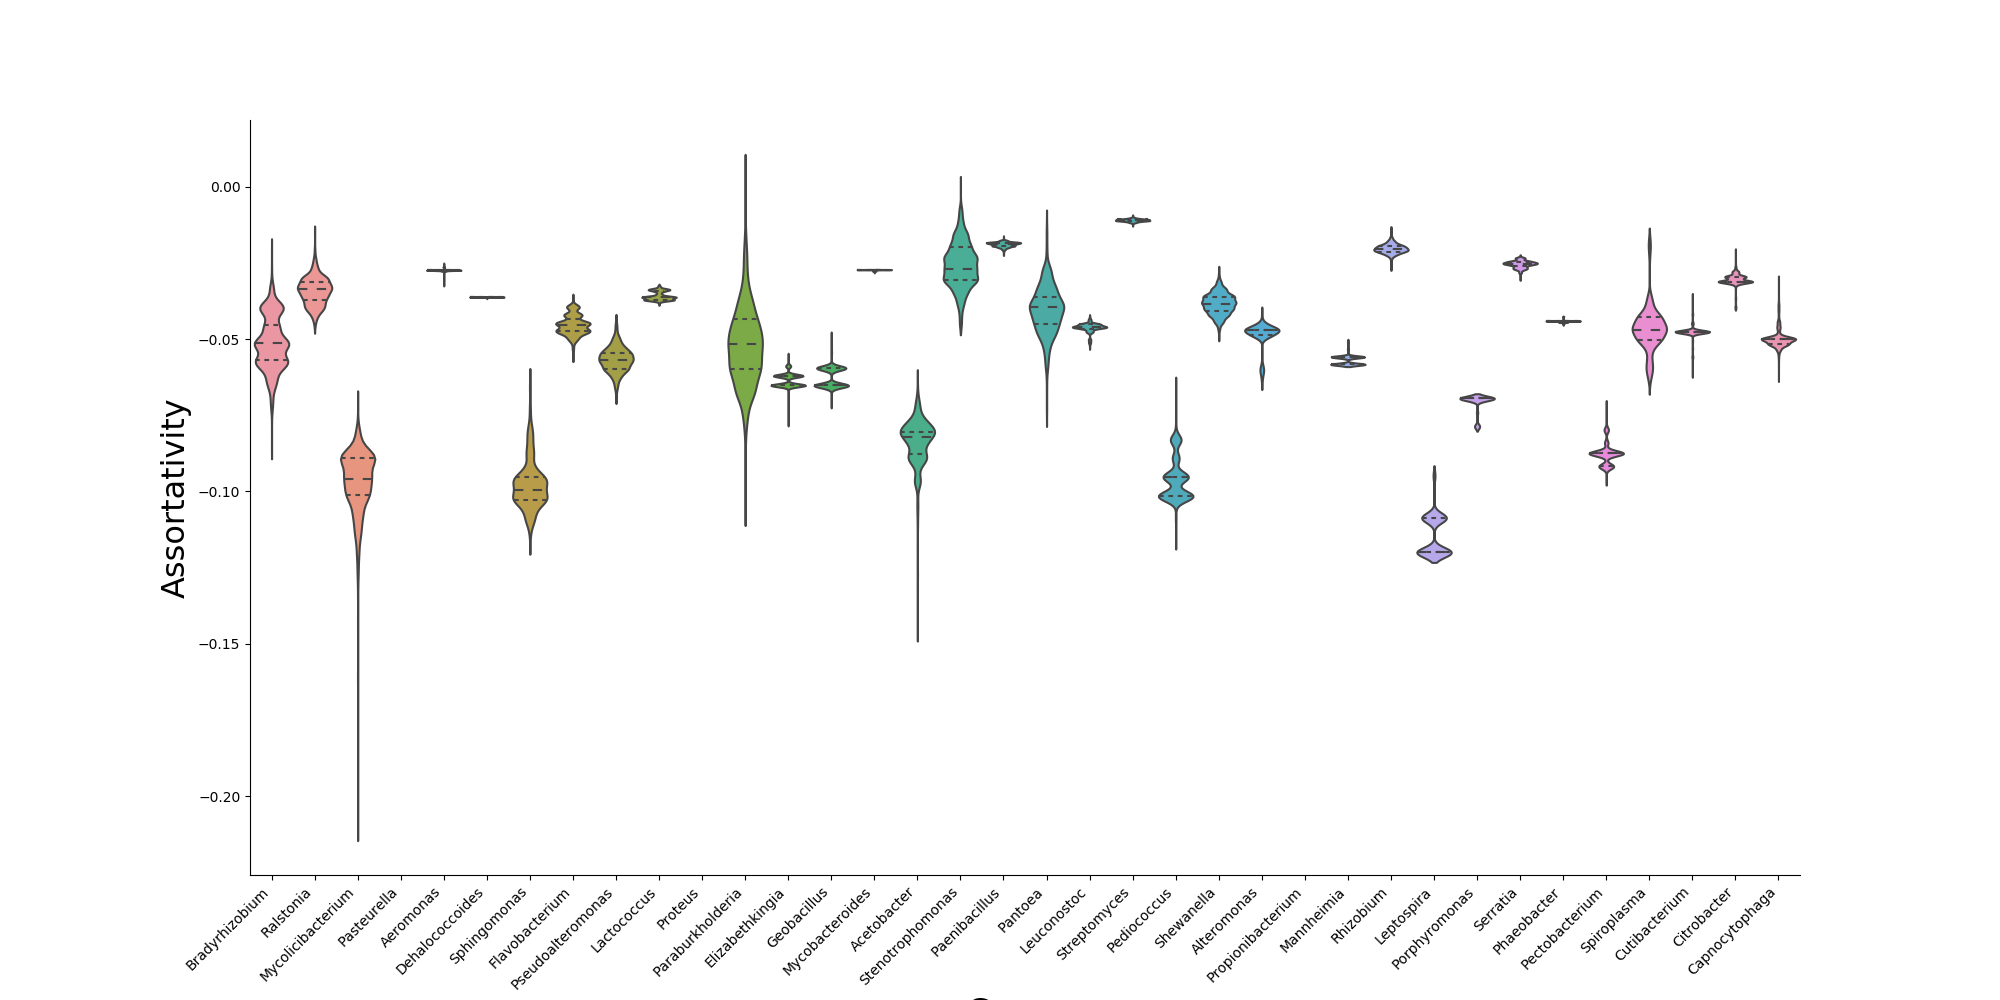
\includegraphics[width=1.2\linewidth]{asst_violin.png}}
    \end{figure}
\end{frame}
\begin{frame}[fragile]{Modularity Distributions}
    \begin{figure}[htb!]
        \makebox[\textwidth][c]{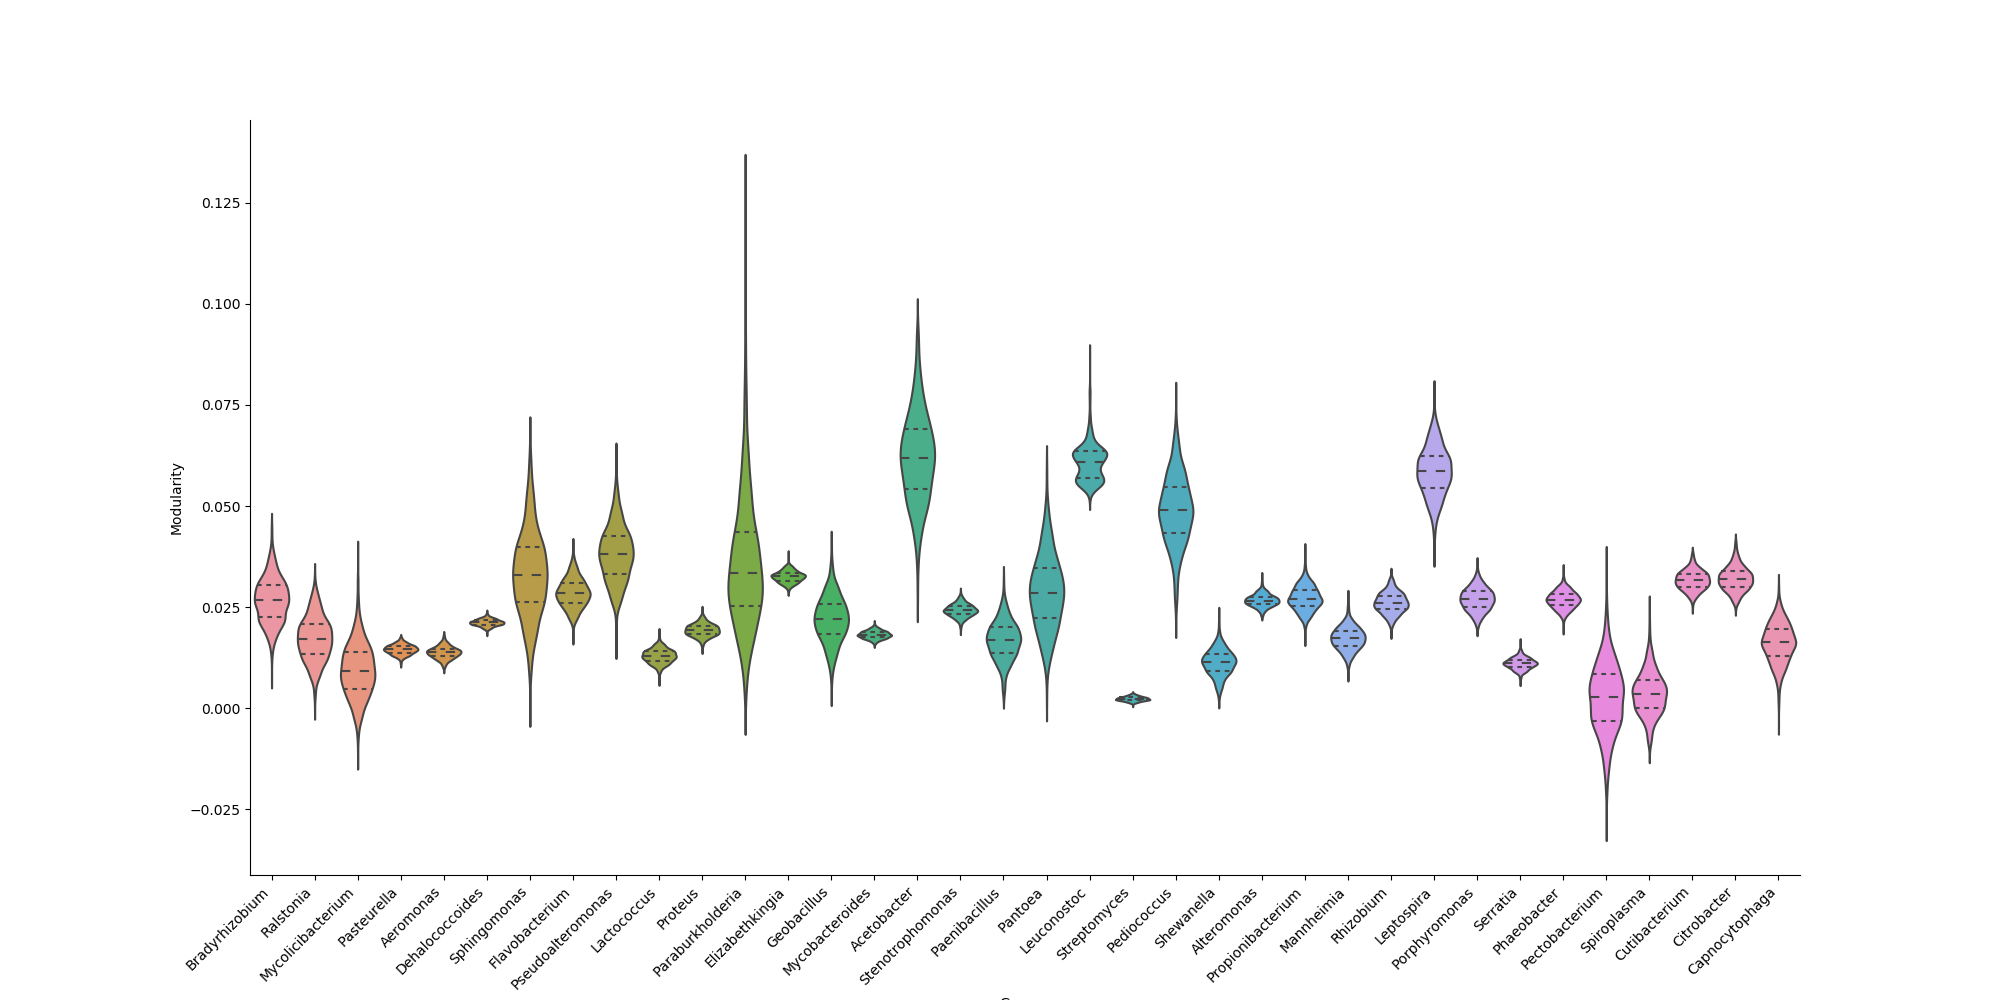
\includegraphics[width=1.2\linewidth]{mod_violin.png}}
    \end{figure}
\end{frame}
\begin{frame}[fragile]{Indel Rate Pair Plot}
    \begin{figure}[htb!]
        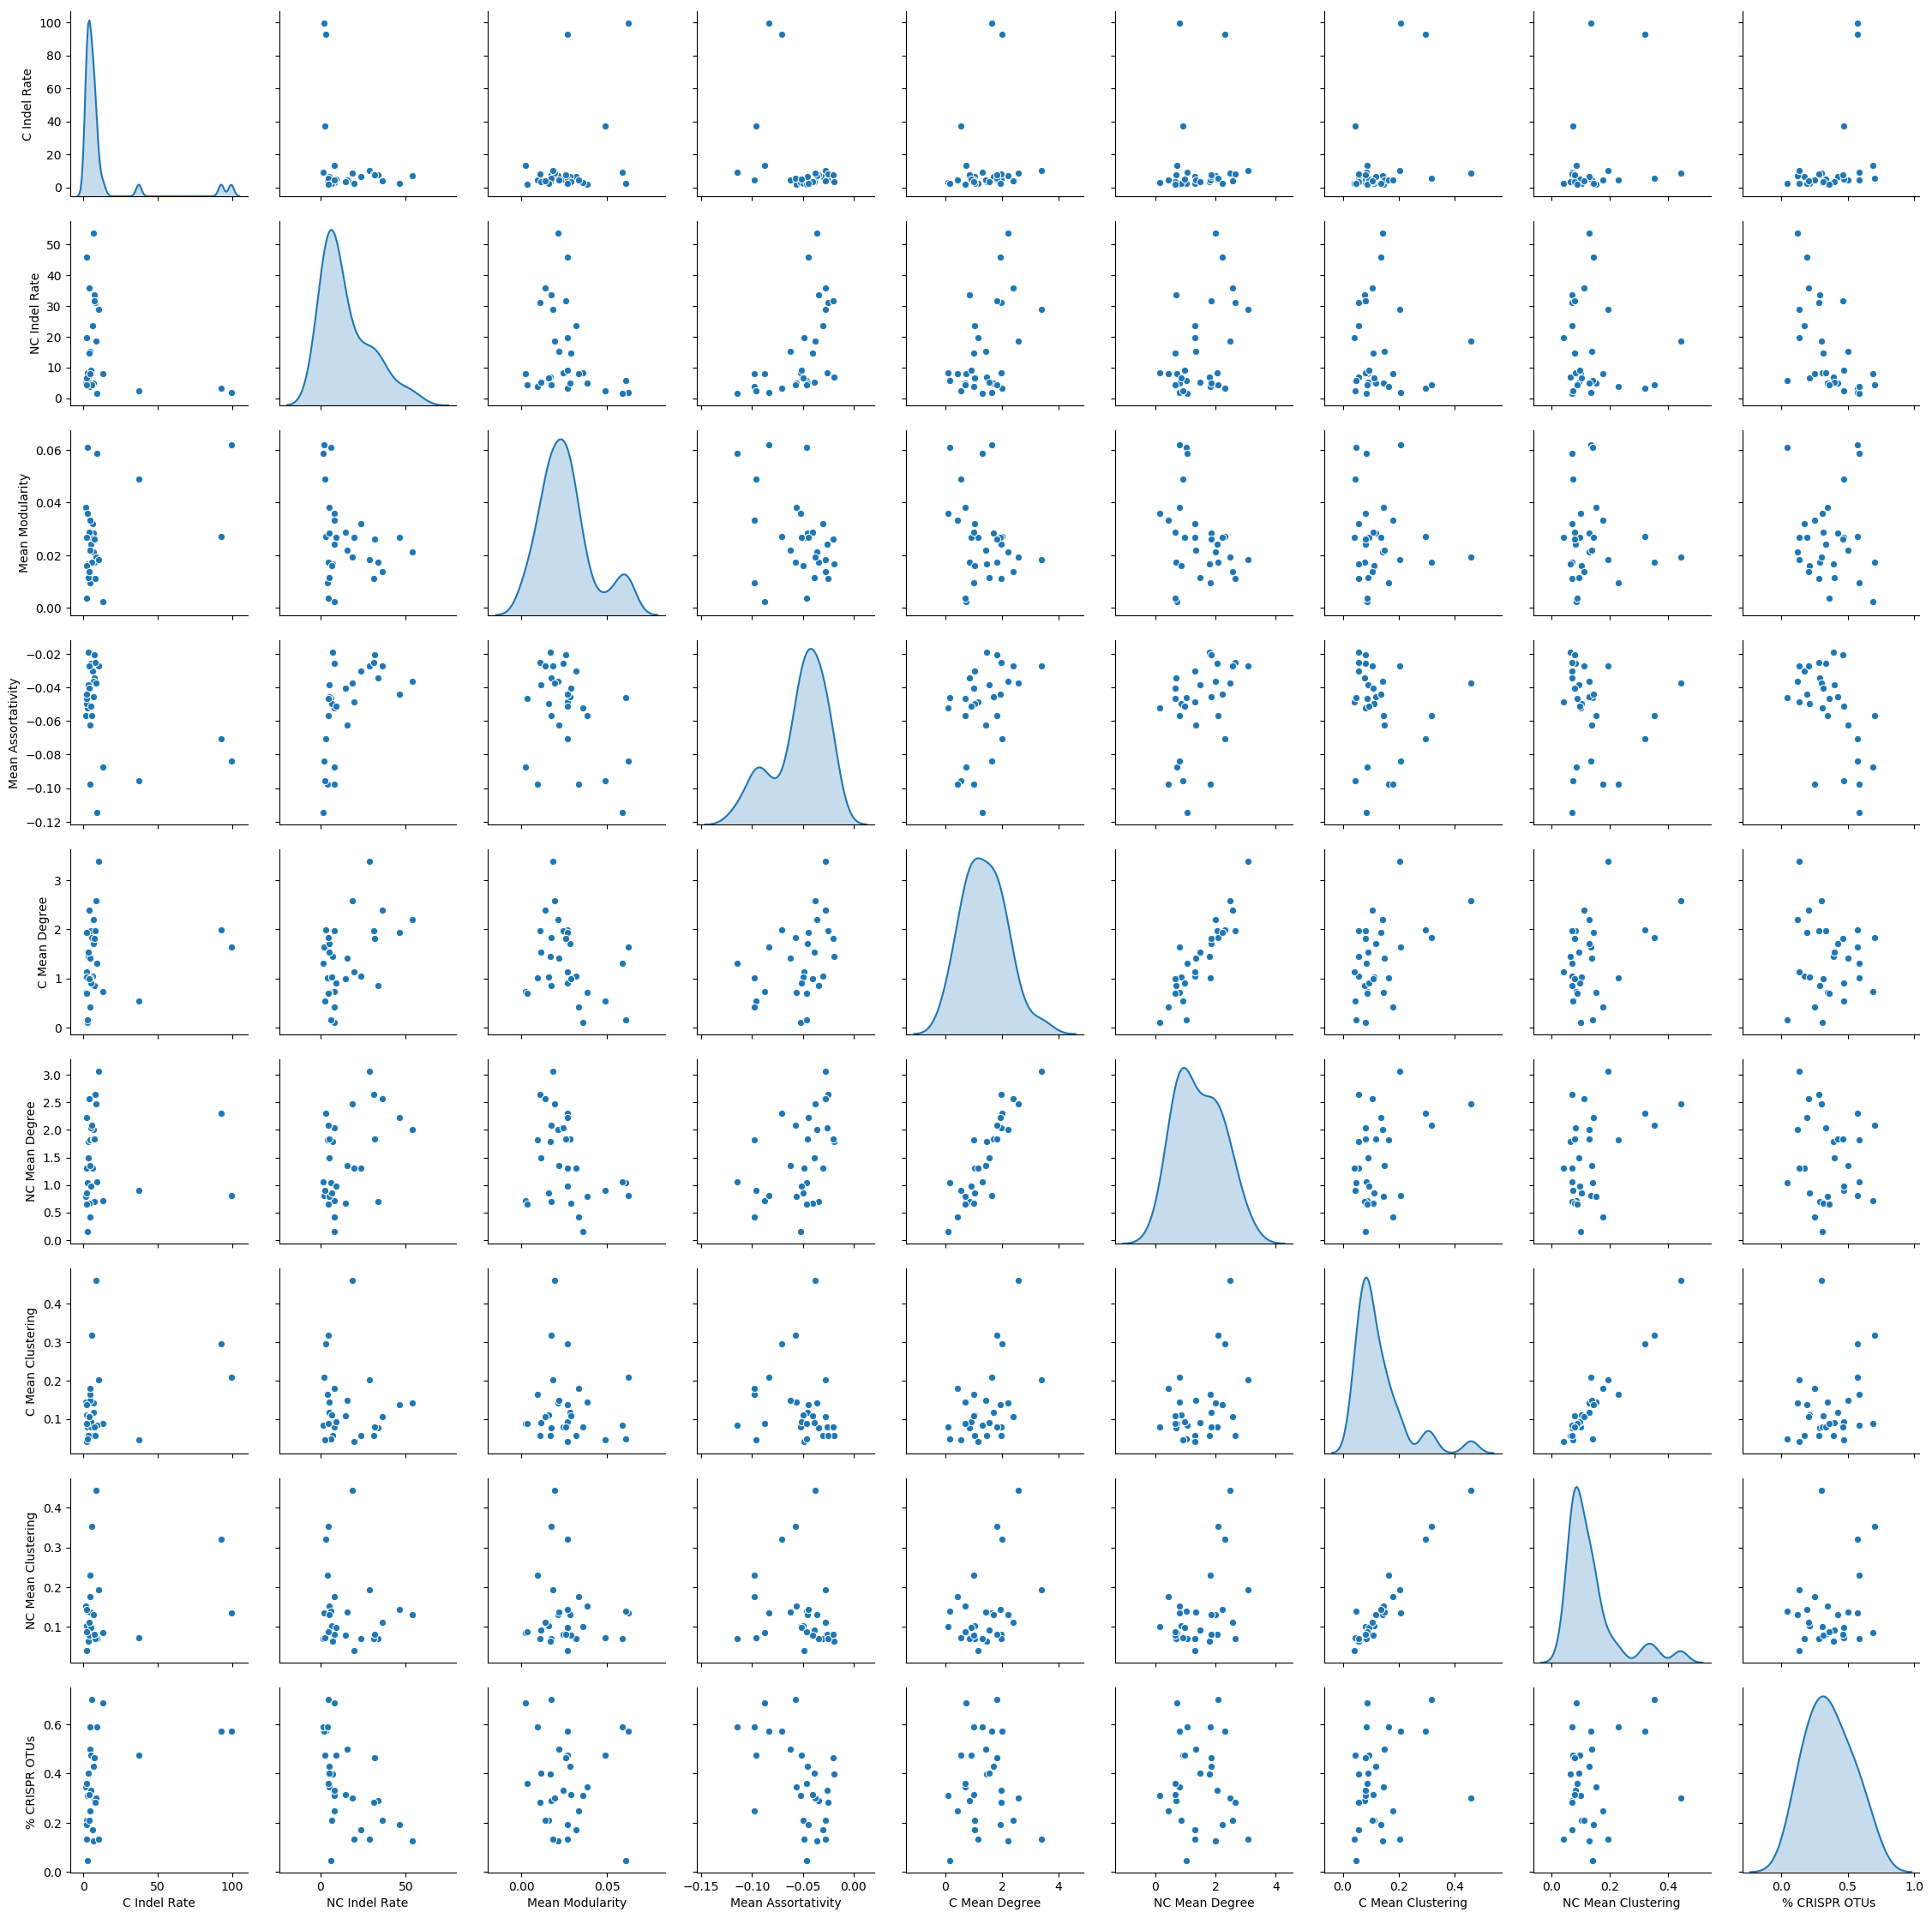
\includegraphics[width=0.6\linewidth]{pairplot.png}
    \end{figure}
\end{frame}
% References
\begin{frame}[allowframebreaks,plain]{References}
    \printbibliography
    \addtocounter{framenumber}{-5}
\end{frame}
\backupend
\end{document}
